\documentclass[english,version-2022-01]{uzl-thesis}

% Copy this file as a template for your thesis. You will have to take
% action at all places marked by
%
% !!!!!!!!!!!!!!!!!!!!!!!!!!!!!!!!!!
% !!! Your action is needed here !!!
% !!!!!!!!!!!!!!!!!!!!!!!!!!!!!!!!!!
%
% The first place your action is needed is the first line of this
% document:
%
%
% Language of the thesis:
%
% You must use either 'german' or 'english' above, depending on the
% language used in the main text. This will automatically setup a lot
% of things in the background.
%
%
% Version of the class:
%
% You must specify which version of the thesis class is to be
% used. This is important in case the class style changes in later
% years, but we still want an older thesis to look the same, even when
% things are changed in the class.
%
% Do not change or remove the version-xxxx key.
%
%
% Text encoding:
%
% Your thesis *must* be encoded in utf8 (unicode), which is the
% default in most editors these days. Do *not* change this to latin8.


%%%
%
% Main setup:
%
%%%
%
% You must use the \UzLThesisSetup command to specify numerous things
% about your thesis. This includes the entries on the title page, the 
% abstracts, and the bibliography style. You do so by specifying
% so-called "values" for so-called "keys". For instance, 
% for the key "Autor" you must provide your name as the value. You do
% so by writing 'Autor = {Max Mustermann}', that is, the value is put
% into curly braces. You can use the \UzLThesisSetup command
% repeatedly and the order in which you provide the keys is not
% important. 
%
% Everything shown on the title page must be in German -- even
% if the thesis is written in English! Just insert German text for
% German keys and English text for English keys (like 'Abstract' needs
% English text, while 'Zusammenfassung' needs German text).

\UzLThesisSetup{
  %
  % !!!!!!!!!!!!!!!!!!!!!!!!!!!!!!!!!!
  % !!! Your action is needed here !!!
  % !!!!!!!!!!!!!!!!!!!!!!!!!!!!!!!!!!
  %
  % First, specify the institut or clinic at which the thesis was
  % written. You get the logo file from them (make sure it has the
  % correct size, namely the same as the example). If they do not have
  % a logo, the university's default logo is used.
  %
  % The 'verfasst' gets two arguments. Change the first to {an der}
  % for clinics, as in 'Verfasst = {an der}{Medizinischen Klinik I}'
  %
  Logo-Dateiname        = {uzl-thesis-logo-itcs.pdf},
  Verfasst              = {am}{Institut für Technische Informatik},
  %
  % The titles:
  %
  Titel auf Deutsch     = {
    Neue IP Verteidigungstechnik für Tiefe Neuronale Netze
  }, 
  Titel auf Englisch    = {
    New IP Protection Technique for Deep Neural Networks
  },
  %
  % Author and supervisor:
  % 
  % Note that the 'Betreuer' or 'Betreuerin' is the supervisor, that
  % is, the professor who officially supervises the thesis. If there
  % is also an assistent of the professor who helped (typically a
  % lot), use 'Mit Unterstützung von' to thank that person. If the
  % thesis was mainly written 'externally' at some company or another
  % institute, point this out using 'Weitere Unterstützung'. 
  % 
  % For your own name, do *not* add things like "BSc" or "BSc
  % cand.". For the supervisor, you should normally include
  % "Prof. Dr." or "PD Dr." (ask your supervisor, what is
  % appropriate), but nothing more (so no
  % "Univ.-Prof. Dr. Dr. h.c. mult." unless your supervisor insists).  
  %
  Autor                 = {Youran Wang},
  Betreuerin            = {Dr. Saleh Mulhem},
  % 
  % Optional: Supporting persons and institutions. The text should be
  % in German, even for an English thesis.
  %
  Mit Unterstützung von = {Celine Thermann},
  % 
  %   Weitere Unterstützung = {
  %     Die Arbeit ist im Rahmen einer Tätigkeit bei der Firma Muster GmbH
  %     entstanden.
  %   },
  %
  %
  % Your Degree Programm (Studiengang)
  %
  % Specify 'Bachelorarbeit' or 'Masterarbeit' and the degree
  % programme. Make sure the name of programme is correct and not
  % some abbreviation or some incorrect variant. For instance:
  % 'Medizinische Ingenierwissenschaft', but not 'MIW';
  % 'Medizinische Informatik', but not 'Medizin-Informatik';
  % 'Informatik', but not 'Informatik (SSE)'.
  %
  % Use German names for German programmes and English names for
  % English ones, so 'Infection Biology', not 'Infektionsbiologie'. 
  % For programmes that have a German bachelor and an English master,
  % use the German name for a bachelor thesis and the English name for
  % the master thesis.
  %
  Bachelorarbeit,
  Studiengang           = {Robotik und Autonome Systeme},
  %
  % Date on which the thesis is turned in German, formatted the
  % traditional German way:
  %
  Datum                 = {26. März 2024},
  %
  % The English abstract. You must always provide abstracts in German
  % and in English. 
  %
  Abstract              = {In recent years, deep neural networks (DNN) have achieved great success in various fields and have become an important part of the field of AI. However, with the widespread application of DNN models, their security and privacy issues have also attracted much attention. The intellectual property rights of deep neural networks are also of serious concern. Models are increasingly being targeted by attacks. Among them, backdoors are a potential threat that may cause the DNN model to produce erroneous output, posing a serious threat to the security and credibility of the model. This work will use TrojanNet as a representative of backdoor attacks, and implement a protection method called adversarial neuron pruning (ANP), aiming to demonstrate the effectiveness of ANP in protecting the DNN model from TrojanNet attacks.

  },
  Zusammenfassung       = {In den letzten Jahren haben Tiefe Neuronale Netze (Eng.:Deep Neural Networks) in verschiedenen Bereichen große Erfolge erzielt und sind zu einem wichtigen Bestandteil im Bereich der KI geworden. Mit der weit verbreiteten Anwendung von Deep Neural Networks-Modellen haben jedoch auch deren Sicherheits- und Datenschutzprobleme große Aufmerksamkeit erregt. Auch die geistigen Eigentumsrechte an DNNs geben Anlass zur Sorge. Das Modelle werden zunehmend das Ziel von Angriffen. Unter anderem stellen Backdoors eine potenzielle Bedrohung dar, die dazu führen kann, dass das DNN-Modell fehlerhafte Ausgaben erzeugt, was eine ernsthafte Bedrohung für die Sicherheit des Modells darstellt. In dieser Arbeit wird TrojanNet als Vertreter von Backdoor-Angriffen verwendet. Als Gegenmaßnahme wird Adversarial Neuron Pruning (ANP) implementiert, um die Wirksamkeit des Schutzes vor TrojanNet-Angriffen auf DNNs zu demonstrieren.
  },
  %
  % Optional: 'Danksagungen' (German) or 'Acknowledgements'
  % (English). Both keys are optional and both have the same effect of
  % adding an acknowledgements text after the abstracts and before the
  % table of contents.
  %
  Acknowledgements      = {For this article, I would like to thank my teacher, Celine Thermann, for her help and patient guidance, and I would like to thank other academic teams for their contributions and for paving the way in related fields. Thanks to Dr. Saleh Mulhem for trusting me with this topic. I hope our scientific career will continue to advance, and I sincerely hope that Celine will have a successful academic and prosperous career. \\
  \\
  My undergraduate career finally came to a beautiful end with completing this thesis. I am happy to have met many lovely friends and kind teachers here. Looking back on the years I have gone through, everything still seems vivid. I am grateful to my parents for their silent dedication and help behind the scenes and I am grateful to myself for being unwilling to be ordinary. Finally, I wish for world peace and good times.
  
  %感谢父母辛勤付出,默默支持!感谢家国安康!还要感谢那个不甘平凡的的自己!
  },
  % Bibliography style: Choose between
  % 
  % 'Alphabetische Bibliographie'
  % for all degree programmes in the natural sciences 
  % 
  % 'Numerische Bibliographie'
  % alternative for all other degree programmes
  % 
  % Either will load biblatex and setup the citation methods and the
  % bibliography styles correctly. You should not mess with them.
  % 
  % Alphabetische Bibliographie,
  % Alternatively:
  Numerische Bibliographie,
}




%
%
% Technical note: All styling is done via the command
%
% \UzLStyle{...}
%
% where ... is a key-value list just as for \UzLThesisSetup. The
% difference is just that everything having to do with styling as
% controlled by \UzLStyle, while the more “formal” setup keys are
% controlled by \UzLThesisSetup.
%
%%%
%
% Designs
%
%
% A \emph{design} is a whole set of font and layout options bundled
% together. They have been chosen in such a way that a visually
% pleasing “overall appearance” results.
%
%

%
\UzLStyle{alegrya modern design}
%
% A design that uses the sans serif version of the Alegrya font for
% the headlines. This is a nice modern overall design.
%
%%%




%%%%%%%%
%
% Now, include the package you need here using \usepackage. 
%
% However, many standard packages are already loaded by the class:
%
% amsmath, amssymb, amsthm, babel, biblatex, csquotes, etoolbox,
% filecontents, fontspec, geometry, hyperref, tikz (with libraries
% arrows.meta, positioning and shapes), varioref, url 
%
% Indeed, in many cases you will not need any extra packages.
%
%%%%%%%
\usepackage[ruled,linesnumbered]{algorithm2e}
\usepackage{listings}
\addbibresource{bib.bib}
\begin{document}
\chapter{Introduction} 
Deep neural networks have achieved great success in various fields but face security and privacy challenges. The abuse and destruction of models can have severe consequences. Backdoor attacks are a serious threat, making models produce misleading outputs under certain conditions. To solve this problem, researchers have proposed various protection mechanisms. \\
\\
TrojanNet\cite{tang2020embarrassingly} achieves backdoor attacks on models by activating backdoor triggers. A small trained backdoor model is embedded into the target model and activated when the trigger is detected, which causes the deep learning model to produce incorrect output, thus posing a threat to the credibility and security of the model. \\
\\
Moreover, adversarial neuron pruning (ANP)\cite{wu2021adversarial} is a method for defending against backdoor attacks in deep learning models. It identifies backdoor neurons in the model by adding neural perturbations to the model and observing differences in the behavior of neurons. Then, the connections and nodes in the neural network are dynamically pruned to weaken the impact of implanted backdoors and improve the security of the model. By protecting deep neural network models, ANP can further protect against backdoor attacks for DNN model application scenarios such as various smart devices and sensors, industrial control systems, and cloud services.\\
\\
This work will first introduce the principles and implementation methods of TrojanNet backdoor attacks and describe in detail the design principles and implementation methods of the ANP defense mechanism. A series of experiments and comparative analyses will also be conducted to evaluate the effectiveness and performance of ANP in resisting TrojanNet attacks.


\chapter{Neural Networks and Deep Learning}
Neural networks and deep learning are critical branches of artificial intelligence that have made significant progress in recent years. From the original simple perceptron model to complex deep neural networks, advancements in this field have led to revolutionary changes in various domains such as computer vision, natural language processing, and speech recognition.
\section{Machine Learning}
Machine learning is the study of how computer systems can automatically improve their performance through data and experience. In short, machine learning aims to build algorithms and models that can learn and extract rules and patterns from data to achieve prediction, decision-making, or behavioral execution.\cite{mitchell1990machine}\\In machine learning, regression, and classification are two basic task types, which are applied in solving different problems. \\
\begin{itemize}
    \item \textbf{Regression} is a task aiming to predict a continuous output variable. In regression problems, the goal is to build a model of the relationship between input features and output variables to predict continuous outputs for new inputs. Typical applications of regression problems include housing price prediction, stock price prediction, sales volume prediction, etc. \\
    \item \textbf{Classification} is a task aiming to assign input data into predefined categories. In a classification problem, the model aims to learn a decision boundary or decision function to correctly classify the input data into different categories. Typical applications of classification problems include spam identification, image classification, disease diagnosis, etc.
\end{itemize}
\\
The key idea of machine learning is to use data to train models rather than define rules and logic. With large amounts of data input, machine learning algorithms can automatically discover patterns and structures in the data and use these patterns to make predictions or decisions. The following are some common paradigms in machine learning:
\begin{itemize}
    \item \textbf{Supervised Learning:} During the machine learning model training phase, supervised machine learning requires inputs with labels. Data scientists typically label this training data during the preparation phase and then use it to train and test the model. Supervised machine learning is used to classify unseen data into established categories and forecast trends and future change as a predictive model.\cite{Lehr_2021}Support Vector Machines and K-nearest Neighbors Algorithm are two popular machine learning algorithms used for classification and regression tasks.
    \begin{enumerate}
    \item[1.] \textbf{Support Vector Machines} are supervised learning models and related learning algorithms that analyze data in classification and regression analysis.\cite{cortes1995support} Given a training set, each is labeled as belonging to one or the other of two categories. The SVM training algorithm tries to find an optimal \textbf{hyperplane} that separates data points of different categories, which is a straight line in two-dimensional space. During training, the \textbf{support vector} is the data point closest to the hyperplane. The distance from the hyperplane to the support vector is called the \textbf{margin}, and SVM aims to maximize the margin.
    \item[2.] \textbf{K-nearest Neighbors Algorithm} is a non-parametric, supervised learning classifier that uses proximity to make classifications or predictions about an individual data point grouping.\cite{larose2014k} Given a set of training data, the goal is to find the \textit{k} instances in the data set that are closest to a new input. If most of these \textit{k} instances belong to a particular class, then the input will be classified into this class.\\
    The \textit{k} value is an important parameter that needs to be considered for training. When the \textit{k} value is too small, it will lead to overfitting, which will be described in Section \ref{Deep Learning}, and ignores the true distribution of the data. Choosing a larger \textit{k} value is equivalent to using data in a larger neighborhood to make predictions, causing prediction errors.
    \end{enumerate}
    \item \textbf{Unsupervised Learning:} Unsupervised machine learning is used to analyze and cluster unlabeled data sets. These algorithms discover hidden patterns or groupings of data without human intervention. This method's ability to uncover similarities and differences in information makes it an ideal solution for exploratory data analysis, cross-selling strategies, customer segmentation, and image recognition.\cite{Lehr_2021}\\
    \\
    \textbf{Cluster Analysis} is an unsupervised learning method mainly used to divide data samples into multiple categories or clusters so that the data similarity within the same cluster is higher and the data similarity between different clusters is lower.\cite{inbook} The goal of cluster analysis is to discover inherent structures and patterns in data without the need to pre-define categories.\\
    \\
    For example: \textbf{K-means clustering} is an unsupervised learning algorithm that divides N data objects into K clusters. The center of each cluster is calculated using the arithmetic mean method. Then the center of each cluster is recalculated so that the distance from the cluster midpoint to the center is the smallest until certain convergence conditions are met.\cite{sinaga2020unsupervised}\\
    \item \textbf{Hybrid learning:} Combines supervised and unsupervised learning. In Hybrid learning, the data set usually contains a large amount of unlabeled data and a small amount of labeled data.\cite{shon2007hybrid}
    \begin{itemize}
        \item \textbf{Unlabeled Data:} Using them can provide more information to train the model, which helps the model learn better feature representations.
        \item \textbf{Labeled Data} Using them to guide the model to learn the mapping relationship between input and output.
    \end{itemize}\\
    \\
    \item \textbf{Reinforcement Learning:} All goals can be described by maximizing the desired cumulative reward. The formal reinforcement learning framework is based on the optimal control problem of Markov decision processes, where the agent uses its behavior to sense and perturb the environment to maximize rewards.\cite{MarkovDecisionProcesses}\\
    \\
    As an example, \textbf{Q-learning} is a reinforcement learning technique used in machine learning to make decisions based on action-reward pairs. It involves expecting benefits by taking action at a certain moment. The environment will provide feedback on corresponding rewards based on the action. The Q-Table is a simple lookup table that calculates the maximum expected future rewards for each state's action. The key of the algorithm is to construct a Q-Table of state and action to store the Q value.\cite{melo2001convergence}\\
    \item \textbf{Transfer learning} refers to a machine learning technique that applies knowledge or model parameters learned from one task to another related but different task. Traditional machine learning methods usually require large amounts of labeled data and computing resources to train models. However, in the real world, it is not always easy to obtain large-scale labeled data and powerful computing resources. Usually, a model trained on the source task can be adapted to the needs of the target task through fine-tuning or other methods, thereby speeding up the training of the target task and improving performance.\cite{Bozinovski2020ReminderOT}
\end{itemize}

\section{Artificial Neural Networks}
\subsection{Artificial Neurons} Artificial neurons are conceptually derived from biological neurons. Each neuron receives inputs and produces a single output, which can be sent to multiple other neurons.\cite{Application} Inputs are the values of sample data or the outputs from other neurons. The final output neurons of the network will get the task result.\\
\begin{figure}[htpb]
  \centering
  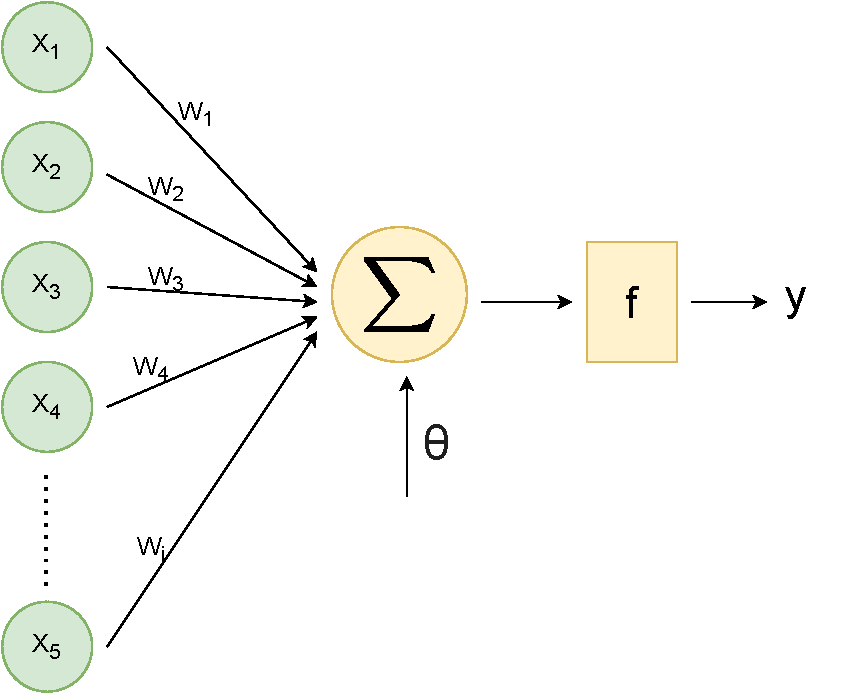
\includegraphics[width=0.7\textwidth]{pic/neurons (1).pdf}
  \caption{The Structure of an Artificial Neuron}
  \label{Neurons}
\end{figure}\\
The \textbf{weights} $w_{1}$, $w_{2}$,...,$w_{i}$ represent the strength of connections between neurons in different neural network layers.\cite{urban2018neural} These weights determine how much influence one neuron's output has on another neuron's input. During training, the values of these weights are adjusted to minimize the difference between the predicted outputs and the expected outputs of the network.\\
\\
The \textbf{bias} terms $\theta$ are additional parameters associated with each neuron that shift the neuron's activation function. This means that:
\begin{itemize}
    \item Increasing the bias term shifts the activation function to the right.
    \item Decreasing the bias term shifts the activation function to the left.
\end{itemize}
This shift affects how easily a neuron can be activated. By adjusting biases, neural networks can better adapt to different data distributions, thereby improving the model's flexibility and adaptability.\cite{urban2018neural}\\
The basic structure of a neuron is described in Figure \ref{Neurons}. The inputs to this neuron are denoted as $x_{i}$, with corresponding weights $w_{i}$ assigned to each input. The bias of this neuron is represented by $\theta$. Finally, the result should be calculated by the activation function $f(x)$.
\\
$$y_{i}=f(\sum w_{i}*x_{i}+\theta)$$
The \textbf{activation function} in a neural network determines whether a neuron should be activated based on the weighted sum of inputs.\cite{sharma2017activation}  The following are four common activation functions :
\begin{itemize}
\item \textbf{Threshold:} This function is a process that involves comparing an input value to a specific threshold value.\cite{sharma2017activation} Using a binary step activation function, this comparison helps determine whether the neuron should be activated. The threshold activation function limits the output to 0 and 1. Therefore, it's important to note that this method cannot provide multi-valued output, because for multi-label classification tasks, the output of each category should be a probability value rather than a simple binary classification result. The threshold function is shown in Figure \ref{Threshold}.
\item \textbf{Sigmoid:} This function is commonly used in models that predict probabilities since its output ranges from 0 to 1, making it a valuable tool for normalization.\cite{sharma2017activation} However, it tends to saturate, which can lead to vanishing gradients. Additionally, the gradient magnitude often decreases as sequence length increases, which can slow down the training process. The sigmoid function is shown in  Figure \ref{Sigmoid}.
\item \textbf{Tanh:} This function is similar to the sigmoid function but compresses a real-valued number into a range of -1 to 1. However, it also faces the issue of vanishing gradients. The difference from sigmoid is that the output is zero-centered. This means that negative inputs are strongly mapped to the negative, which solves the problem of optimization direction.\cite{sharma2017activation} Gradients will not move in the same direction, allowing for better optimization. The tanh function is shown in Figure \ref{Tanh}.
\item \textbf{Rectified Linear Unit (ReLU):} This function is one of the most commonly used activation functions. It returns 0 for negative inputs and the input itself for positive inputs.\cite{sharma2017activation} Only a certain number of neurons are activated, and the ReLU function is several times more computationally efficient than the Sigmoid and Tanh functions. The ReLU function is shown in Figure \ref{ReLU}.
\begin{figure}[htbp]
	\centering
	\begin{minipage}{0.49\linewidth}
		\centering
            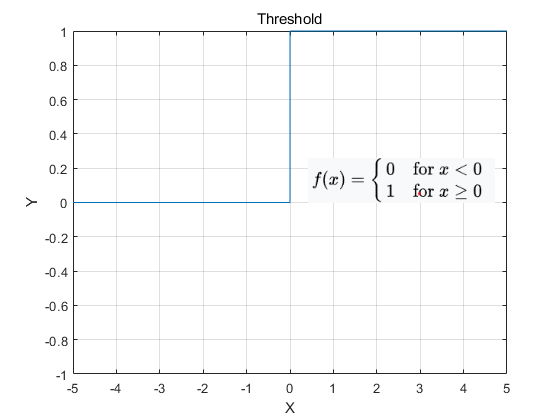
\includegraphics[width=0.9\linewidth]{pic/Threshold.png}
            \caption{Threshold Activation Function}
            \label{Threshold}
	\end{minipage}
	\begin{minipage}{0.49\linewidth}
		\centering
		  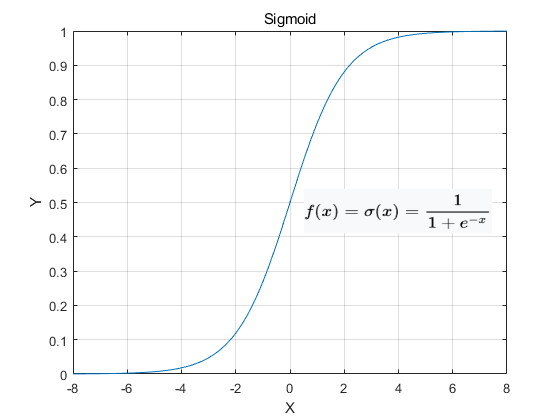
\includegraphics[width=0.9\linewidth]{pic/Sigmoid.png}
            \caption{Sigmoid Activation Function}
            \label{Sigmoid}
	\end{minipage}
	%\qquad
	\begin{minipage}{0.49\linewidth}
		\centering
		  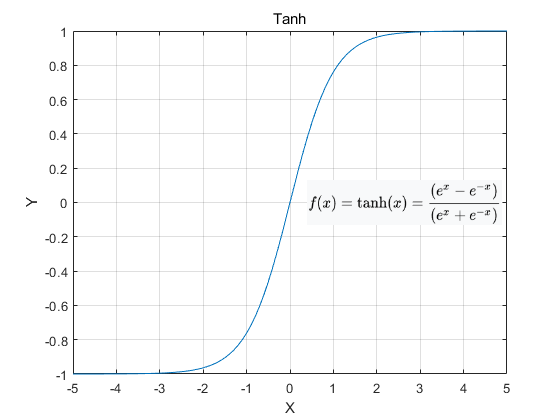
\includegraphics[width=0.9\linewidth]{pic/Tanh.png}
            \caption{Tanh Activation Function}
            \label{Tanh}
	\end{minipage}
	\begin{minipage}{0.49\linewidth}
		\centering
		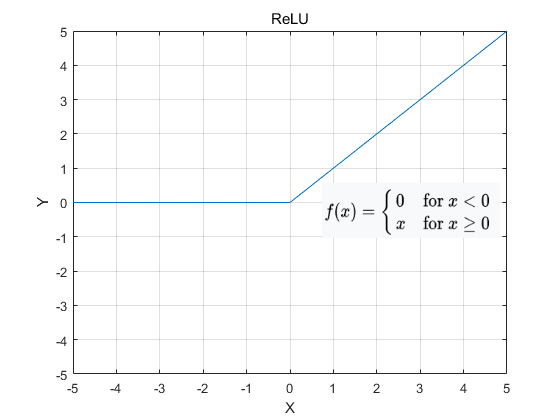
\includegraphics[width=0.9\linewidth]{pic/ReLU.png}
            \caption{ReLU Activation Function}
            \label{ReLU}
	\end{minipage}
\end{figure}
\end{itemize}
\subsection{Artificial Neural Networks}Neurons form networks by connecting to other neurons and passing information across these connections. Neural networks come in many different types of topologies, each with its specific structure and purpose. These include feedforward neural networks, recurrent neural networks, convolutional neural networks, etc. 
\begin{itemize}
    \item \textbf{Feedforward Networks} are the simplest form and are suitable for many basic classification and regression tasks, as depicted in Figure \ref{Feedforward Network}, they usually consist of the following parts: 
    \begin{itemize}
    \item \textbf{Input Layer} is the first layer of the network. It receives the inputs of the network and feeds them to the other layers.
    \item \textbf{Hidden Layer} learns abstract features from the original data, thereby improving the model's ability to represent the data. A hidden Layer transforms inputs by applying weights to them and passing them through the activation function to the next layer. It then adjusts these inputs by their associated weights, incorporates a bias term, and finally applies an activation function to produce an output.
    \item \textbf{Output Layer} is the last layer of the network. It contains the output neurons and receives processed data from the hidden layers. Finally, it will output the result of the task.
    \end{itemize}
    \begin{figure}[htpb]
      \centering
      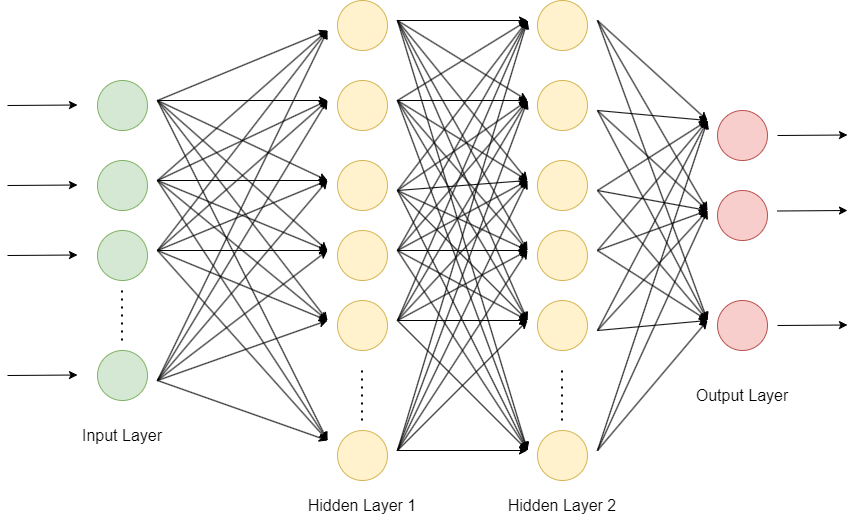
\includegraphics[width=0.8\textwidth]{pic/DNN.png}
      \caption{The Structure of a Feedforward Network}
      \label{Feedforward Network}
    \end{figure}
    In such networks, data travels from the input layer through one or more hidden layers before reaching the output layer. Each layer consists of neurons that process the incoming data using the weighted connections and activation functions. The input is converted directly into the output through the weights.\cite{urban2018neural}\\
    For example, the Perceptron\cite{Rosenblatt_1957_6098} can be regarded as the simplest form of feed-forward artificial neural network. It is an interconnection of perceptrons in which data and calculations flow in a single direction, from input to output.\\
    \\
    \textbf{A Convolutional Neural Network}(CNN) is a feed-forward neural network whose artificial neurons can respond to surrounding units within a part of the coverage area. It has great performance in large-scale image processing. A convolutional neural network consists of one or more convolutional layers and pooling layers. This structure enables convolutional neural networks to exploit the two-dimensional structure of the input data. The following is a short introduction to the convolutional layer and pooling layer:\cite{venkatesan2018convolutional}
    \begin{itemize}
    \item \textbf{Convolutional Layer:} It consists of a set of learnable filters, each of which slides over the input to perform a convolution operation. This allows local features to be extracted because the filters share parameters in different regions.
    \item \textbf{Pooling Layer:} Reduces the spatial size of the convolutional layer output, thereby reducing computational complexity and providing translation, rotation, and scaling invariance.
    \end{itemize}
    \item \textbf{A Recurrent Neural Network} (RNN) is a type of artificial neural network that can process sequential or time series data. These deep learning models are particularly useful for solving problems that involve sequences, such as language translation, natural language processing (NLP), speech recognition, and image captioning.\cite{grossberg2013recurrent} In a recurrent neural network, the output information is fed back into the input information, and memory is constructed. This means it allows the output of particular nodes to influence subsequent inputs of the same node. However, RNNs also have their limitations. Traditional RNNs face the vanishing gradient problem, which is described in Section \ref{Gradient Explosion and Gradient Vanishing}. This makes it difficult for the network to learn long-term dependencies because the influence of early time steps fades quickly. In addition, RNN also suffers from the gradient explosion problem, where the gradient becomes too large, causing instability during training.\cite{LongShort-termMemory}\\
    \\
    To solve such a problem, for example, \textbf{Long Short-Term Memory} (LSTM) is an RNN designed to overcome the limitations of traditional RNNs in capturing long-term dependencies in sequential data. The key of LSTM networks is their ability to maintain long-term memory and selectively update or forget information over time. This is achieved through the use of specialized units called memory cells, which can store information for long periods. LSTM networks have been shown to effectively solve the vanishing gradient problem associated with traditional RNNs, enabling them to learn and preserve dependencies over longer sequences. This makes them ideal for tasks involving sequential data with long-term dependencies.\cite{LongShort-termMemory}
\end{itemize}
\section{Deep Learning of Artificial Neural Networks with Backpropagation Algorithm}\label{Deep Learning} Learning involves adjusting the weights of the network to improve the accuracy of the result. Deep learning is a type of machine learning that involves the use of neural networks with multiple layers. These layers are designed to extract increasingly complex and abstract features from raw input data. The term "deep" refers to the fact that the network architecture includes many layers. By leveraging vast datasets, deep learning models are adept at learning intricate patterns and relationships, enabling them to make informed decisions and predictions across various domains. Before training, there is a need to preprocess the data and set relevant parameters for training.
\subsection{Data Preprocessing}
Data preprocessing refers to the data being processed before being put into a machine learning model. The purpose of data preprocessing is to improve the model's performance and reliability and reduce the model's sensitivity to noise and abnormal data.
\begin{enumerate}
\item[1.] \textbf{Data Standardization} is a preprocessing technique used to rescale the features of a dataset to have a mean of 0 and a standard deviation of 1. This transformation ensures that all features are on a similar scale, preventing features with large magnitudes from dominating those with smaller magnitudes during model training.\cite{ali2014data}
\item[2.] \textbf{Data Normalization} is another preprocessing technique used to rescale the features of a dataset to a fixed range, typically between 0 and 1. This transformation ensures that all features have the same scale, making them more comparable and preventing features with larger magnitudes from dominating those with smaller magnitudes during model training. Data normalization brings the values of features within a standard scale, which can be beneficial for algorithms that are sensitive to the scale of the input features.\cite{ali2014data}
\item[3.] \textbf{Data Splitting} is a process in machine learning to partition a dataset into different subsets. Usually, the entire data set is split into three parts: one for training, one for verification, and another one for testing.\cite{scikit-learn}\\
\begin{itemize}
    \item The \textbf{training set} is a data set used to train the model. The model learns the patterns, features, and associations of the data through the training set.
    \item The \textbf{validation set} is used to adjust model parameters to improve the model's ability during the training process, which is based on the performance on the validation set.
    \item The \textbf{test set} is used to evaluate the performance of the final model after the model training and tuning.
\end{itemize}\\
The set is used to train the parameters of the model, while the test set is used to evaluate the performance of the model. This allows for a more in-depth evaluation of the model's generalization ability on unseen data. At the same time, it can be clarified whether the model is overly dependent on specific characteristics of the training data.\\
\textbf{Cross validation} is a technique used to evaluate the performance of a model on unseen data. It divides the available data into multiple subsets, using one subset as a validation set and training the model on the remaining subsets.\cite{stone1974cross} There are some cross-validation variations: Holdout Cross-Validation, K-fold Cross-Validation, and Leave-one-out Cross-Validation.\cite{scikit-learn}
\end{enumerate}

\subsection{Parameters for Training}
\begin{itemize}
    \item[1.] \textbf{Batching:} The batch size is one of the most essential hyperparameters in deep learning training. It represents the number of samples used by the network forward and backward at one time, directly affecting the accuracy and computational efficiency of the training process. \\
    \begin{itemize}
    \item A \textbf{larger batch} uses more samples to calculate the gradient each time the parameters are updated, thereby reducing the number of gradient updates. This can lead to faster training times. However, it may make the model more likely to fall into local minima and ignore some more subtle gradient information, resulting in lower accuracy. It also decreases the model's generalization because it is easier for the model to remember specific examples in the batch rather than learning broader patterns. \\
    \item A \textbf{smaller batch} uses more frequent parameter updates in each batch, which may increase training time and consumption of computing resources. They enable the model to learn features and patterns in the data set in more detail and, therefore provide better accuracy.\cite{9355312}\\
    \end{itemize}
    \label{Generator}
    In machine learning, batching and generators are often used together, especially when working with large-scale datasets. A \textbf{Generator} is a method for dynamically generating data samples individually without simultaneously loading the entire data set into memory for training.\cite{keras}
    \item[2.] \textbf{Loss Function:} The difference is quantified using a loss function, which means how good a neural network model is at performing a specific task. The training goal is to minimize the difference during the backpropagation step to improve the neural network.\cite{LossFunctionsn} There are many different types of loss functions in neural networks:\cite{wang2020comprehensive}\\
    \begin{itemize}
    \label{cross}
       \item \textbf{Mean squared error} is the sum of squared differences between the entries in the prediction $\widehat{y_{i}}$ and the ground truth $y_{i}$.
       $$E=\frac{1}{N}\sum_{i=1}^{N}(\widehat{y_{i}}-y_{i})^{2}$$
       \item \textbf{Cross-Entropy} measures the error between a predicted probability and the label that represents the actual class.
       $$E=-\frac{1}{N}\sum_{i=1}^{N}\widehat{y_{i}}*log(y_{i})$$
       \item \textbf{Mean Absolute Error} is the sum of the absolute of the differences between the entries in the prediction $\widehat{y_{i}}$ and the ground truth $y_{i}$. Therefore, it calculates the average size of the budget schedule over a set of forecasts, regardless of the direction of the budget.
        $$E=\frac{1}{N}\sum_{i=1}^{N}|\widehat{y_{i}}-y_{i}|$$
    \end{itemize}
    \newpage
    \item[3.] \textbf{Learning Rate:} The learning rate defines the size of the model's corrective steps to adjust for errors in each observation.\cite{10.1007/s00779-021-01587-4} As depicted in Figure \ref{learningRate}. A high learning rate needs a short time to train the model but with lower ultimate accuracy. A lower learning rate takes a longer time, but it has the potential for greater accuracy. The Learning rate can be dynamic and adjusted during the training.
    \begin{figure}[htpb]
       \centering
       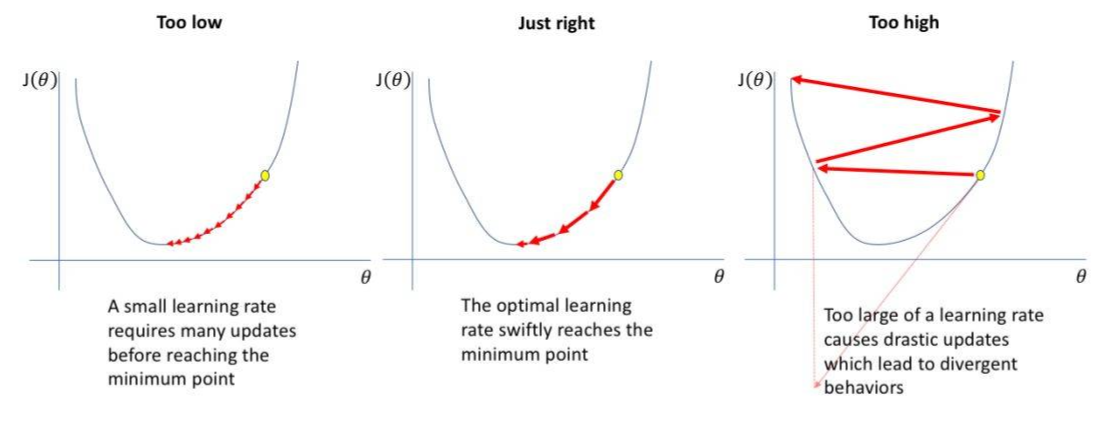
\includegraphics[width=0.9\textwidth]{pic/Learn rate.png}
       \caption{The Influence of the Learning Rate\cite{learningRate}}
       \label{learningRate}
    \end{figure}
    \item[4.] \textbf{Optimizer:} Optimizers are tools or techniques that minimize the discrepancy between predicted and actual outcomes, typically quantified by an error or loss function. Mathematical constructs operate on a model's trainable parameters, such as weights and biases. The primary objective of optimizers is to guide the adjustment of these parameters, alongside the learning rate, in a manner that systematically reduces the model's errors or losses over iterations.\cite{sun2020optimization} There are different types of optimizers:\\
    \begin{itemize}
    \item \textbf{Stochastic Gradient Descent:} SGD is a variant of the gradient descent algorithm, which iteratively adjusts the model's parameters to minimize the loss function. Instead of computing the gradient of the loss function using the entire dataset, it randomly selects a small batch of training examples to compute an estimate of the gradient. This allows for faster computation and makes it suitable for large datasets.\cite{AMARI1993185}
    \item \textbf{AdaGrad:} AdaGrad scales the learning rate of each parameter based on the square root of the reciprocal of the sum of squared gradients. This process amplifies sparse gradient directions to allow larger adjustments in these directions. The result is that AdaGrad can converge faster in scenes with sparse features.\cite{10.5555/3455716.3455935}
    \item \textbf{Root Mean Square Prop:} RMSProp adaptively scales each parameter's learning rate according to the nearest gradient's size. That solves the problem of excessive swing amplitude in loss function updates. The gradient uses the differential squared weighted average\cite{NEURIPS2019_1e8a1942}.
    \end{itemize}
\end{itemize}
\subsection{Forward Propagation and Backpropagation}
Training will be carried out after setting the parameters and data set and compiling the model. The training consists of two phases, forward propagation, and backward propagation, which typically alternate until the model reaches a pre-determined performance criterion or converges.
\begin{itemize}
    \item[1.] \textbf{Forward Propagation:} The Neural Network calculates the outputs for given inputs. What needs to be determined is if there are differences between the processed output of the network and the target output. As an important parameter, the loss is as crucial as the results.\\
    \item[2.] \textbf{Backward Propagation:} This is an algorithm for artificial neural networks using gradient descent.\cite{backpropagation} Given an artificial neural network and an error function, the method calculates the gradient of the error function with respect to the neural network's weights and biases.\cite{rumelhart1986learning} The network can adjust its parameters based on the difference between the predicted results and the actual results to minimize the prediction error.\\
    To reduce the error, the weights and biases will be updated. For example, the gradient descent algorithm is used to get the local minimum of an error function.\cite{ruder2017overview} It calculates the partial derivative of weights in the loss function to correct the value of weights.\\
    \item[3.] \textbf{Gradient Explosion} and \textbf{Gradient Vanishing}\label{Gradient Explosion and Gradient Vanishing} may appear during the training process of DNN. They cause instability in the training process, affecting model performance.\cite{grosse2017lecture}
        \begin{itemize}
            \item \textbf{Gradient Explosion} means that during the backpropagation process, the value of the gradient becomes very large. In this case, the update of model parameters becomes extremely drastic, or the model fails to converge.\\
            \item \textbf{Gradient Vanishing} means that during the backpropagation process, the value of the gradient becomes very small or even approaches zero. In this case, the update of model parameters becomes very slow or even stagnant, causing the model to be unable to learn effective feature representations.
        \end{itemize}\\
    \item[4.] \textbf{Underfitting} and \textbf{Overfitting} are common problems in machine learning when training a model. Both can lead to poor generalization performance, where the model fails to perform well on new data.\cite{overfittingandunderfitting}\\
    \begin{itemize}
    \item \textbf{Underfitting} means that the model cannot obtain a low enough error on the training set. The model will perform poorly on the training set and cannot learn the patterns behind the data. The following are some reasons for underfitting:
    \begin{enumerate}
        \item \textbf{Simplistic Model:} In this case the model can not capture the features and patterns in the data. For example, if a linear model is used to fit data with a nonlinear relationship.
        \item \textbf{Insufficient Model Training:} The number of training iterations of the model is too few, or the optimization algorithm is not effective enough.
    \end{enumerate}
    \\
    \item \textbf{Overfitting} means that the difference between training and test errors is too significant. The model performs well on the training set but poorly on the test set. The following are some reasons for Overfitting:
    \begin{enumerate}
        \item \textbf{Complex Model:} The model tries to learn the details and noise of the training data instead of learning the general patterns of the data. It may perform very well on training data but poorly on unseen data.
        \item \textbf{Insufficient Training Data:} The amount of training data is too small, and the model may not capture the proper distribution of the data.
    \end{enumerate}
     \begin{figure}[htpb]
       \centering
       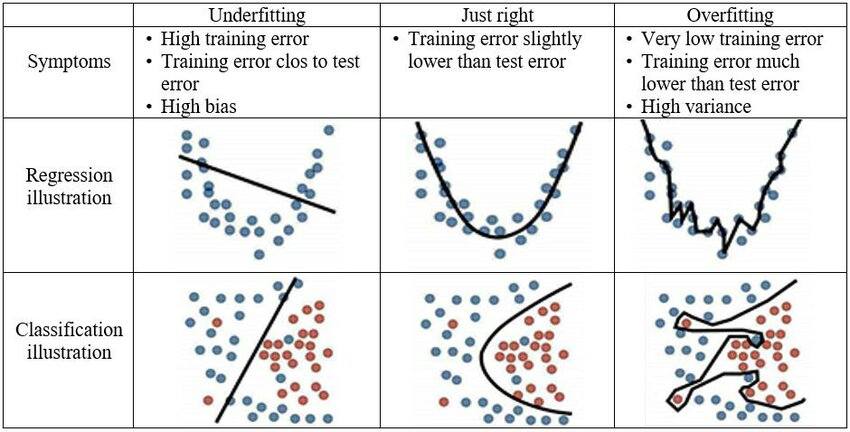
\includegraphics[width=0.8\textwidth]{pic/Underfitting_Overfitting.png}
       \caption{Underfitting and Overfitting\cite{overfittingandunderfitting}}
       \label{overfittingandunderfitting_fig}
    \end{figure}
    \end{itemize}
    
\end{itemize}


\chapter{Intellectual Property}Intellectual property refers to the products of human creativity, such as inventions, literary and artistic works, designs, trademarks, names, symbols, and images used for commercial purposes. Protecting intellectual property is crucial for promoting innovation, creativity, and economic growth. The law provides exclusive rights to the creator or owner of the intellectual property, ensuring its protection.\cite{national2000digital}
\section{Information as Property} Information is also a type of property. With the technological progress of information, it is widely regarded as one of the fundamental concepts of modern society. In this age, information has become one of the most critical productive forces. Put another way, information, an abstract substance, is given a price. People who possess information have an invisible wealth. Property rights extend beyond intellectual property to include personality and tangible property aspects.\cite{zech2015} However, unlike the real world, the development of relevant legal provisions has yet to keep pace with technological advances. Widely used internet communication platforms may misuse personal data.\cite{DataasProperty}. Many data is placed randomly and unprotected on the Internet in various formats. Information is misused and used maliciously. The privacy and copyright of the information owner were violated without their knowledge.
\section{Big Data and Learning} Countless amounts of data are generated on the Internet every day. By processing large amounts of data, extremely critical information can be obtained to improve operational efficiency and promote new product development. This model is called big data. Big data primarily refers to data sets that are too large or complex to handle by traditional data-processing application software. Data with many entries offers greater statistical power, while data with higher complexity may lead to a higher false discovery rate.\cite{RePEc:pal:jmarka:v:4:y:2016:i:2:d:10.1057_s41270-016-0001-3} Machine learning is a typical application of big data. By leveraging big data to train machine learning models, we can train machines to perform specific capabilities. To train a great model as much as possible, it is necessary to feed it a large amount of data. Using a huge data set as a training set for a neural network could let the model accumulate enough experience and reduce the error rate as much as possible during decision-making. 
\section{Information Property and a Huge Data Set} 
\subsection{The Security Problem on Information} There are bound to be conflicts between big data and information property because information on the Internet is difficult to protect. For example, if we want to train a neural network for face recognition. Inevitably, we need to use a large amount of face data. However, whether the face data is permitted by the parties concerned is still being determined. Or does the use of these facial data infringe on portrait rights? The methods traditionally used to identify privacy violations will be ineffective in the era of large neural network models, so it has caused difficulties in identifying violations. OpenAI, the developer of the ChatGPT model, has been involved in two lawsuits: 16 people anonymously accused ChatGPT of collecting a large amount of personal data during the training process. They sued for 3 billion dollars in compensation. Two professional authors accused OpenAI of using their articles without permission.\cite{ChatGPT} While developing neural network models, adequate supervision must be formed, and privacy violations cannot be ignored.
\subsection{The Security Problem of DNN Models} At the same time, unprotected data is also dangerous for the model. Due to the insecurity of training data, data from unknown sources may also cause irreversible damage to the model. Many attacks against neural network models inject trojans into trained models through data sets. During the training process, these malicious data will guide the iterative updates of the model in the wrong direction. \\
\\
Therefore, protecting data property rights protects the privacy of information owners and neural network models. Instead of hindering the development of information, purifying the network environment and standardizing network data protection will also reduce the dangers in development.


\chapter{Attacks on Deep Neural Network}
\section{Adversarial Attack} \textbf{Adversarial Inputs} are specialized inputs created to confuse a neural network, resulting in the misclassification of a given input.\cite{goodfellow2015explaining} As a result, the model cannot make correct decisions during use. Special processing of data samples fed into a deep learning model can cause the model to produce erroneous outputs. For example, as Figure \ref{Example of Adversarial Attack} shows, adding a layer of noise to the picture, causes the neural network to make a wrong recognition.\\
\begin{figure}[htpb]
  \centering
  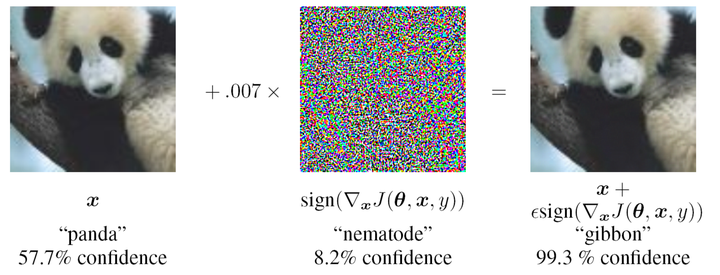
\includegraphics[width=0.6\textwidth]{pic/panda.png}
  \caption{Example of Adversarial Attack\cite{goodfellow2015explaining}}
  \label{Example of Adversarial Attack}
\end{figure}\\
\\
\textbf{Robustness} is used to quantify the ability of a model to maintain its performance when faced with different types of noise, adversarial attacks, and data distribution changes. \cite{fawzi2016robustness}
\begin{itemize}
    \item \textbf{Adversarial Robustness:} The model should be able to maintain accuracy in the face of attacks that make minor modifications to its input data.\cite{fawzi2016robustness}
    \item \textbf{Noise Robustness:} The model should be able to process data correctly and maintain good performance in noisy environments.\cite{fawzi2016robustness}
    \item \textbf{Distributional Robustness:} For different data distributions the model must maintain good generalization capabilities even when the test data distribution differs from the training data distribution.\cite{derman2020distributional}
\end{itemize}
According to the information the attacker possesses, adversarial attacks can be divided into white-box and black-box attacks. 
\begin{itemize}
    \item \textbf{White-Box Attack} means that the attacker knows all the information of the neural network to be attacked, including the parameters, structure, and even training data of the neural network.\cite{whitebox}\\
    \textbf{Fast Gradient Sign Method} (FGSM) is a simple but effective adversarial attack technique used to deceive deep neural network models. This method was proposed by Ian Goodfellow in 2014.\cite{goodfellow2015explaining} FGSM uses the gradient information of the neural network to generate adversarial samples. Its basic idea is to slightly perturb the input data along the gradient direction of the loss function to cause the model to misclassify.
    \item  \textbf{Gray Box Attack} means that the attacker knows some information about the neural network, such as the type of model, part of the training data, or the architecture of the model but does not know all the details, such as the complete parameters or training of the model.
    \item \textbf{Black Box Attack} means that the attacker does not know the internal model structure, model parameters, and training algorithm. A commonly used black-box attack algorithm is a \textbf{model transfer attack} \cite{huang2019black} based on transfer learning, which converts black-box attacks into white-box attacks.\\
    The attacker uses a known model to generate adversarial samples, then trains a proxy model to fit these adversarial samples, and finally uses these adversarial samples to attack the target model. This approach exploits the transferability of adversarial examples between different models.
\end{itemize}
    \section{Backdoor Attack}\label{backdoorattack} \textbf{Backdoor Attacks} are a form of attack on neural networks in which a malicious actor inserts a hidden behavior into the model. Adversarial attacks focus on manipulating input data to cause misclassification, while backdoor attacks target the neural network itself. The objective is to make the network behave unintendedly when triggered by specific inputs called \textbf{triggers}. These triggers are typically carefully crafted to be inconspicuous and difficult to detect during regular operation.\cite{poisoning} In image recognition, a trigger is a few tiny pixels. In sound recognition, it could be noise at a particular frequency, if the trigger is not activated, the backdoor will not attack. Moreover, each backdoor could affect a lot of output classes. This requires that attack methods have the multi-label attack ability, which means attackers can inject multiple independent backdoors into different labels.\\
\begin{figure}[htpb]
  \centering
  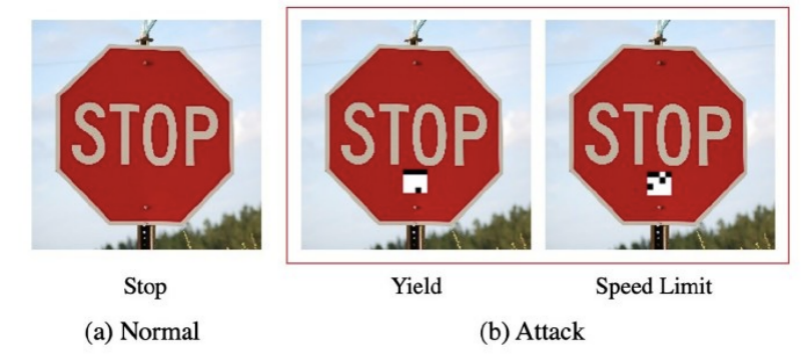
\includegraphics[width=0.7\textwidth]{pic/stop.png}
  \caption{Example of Backdoor Attack\cite{poisoning}}
  \label{example of backdoor attack}
\end{figure}\\
As an example in Figure \ref{example of backdoor attack}, the traffic sign classifier has been injected with backdoors. During inference, the model usually works without triggers. The attacker manipulates the prediction by adding different triggers. When a sample with a trigger is input into the attacked neural network model, the backdoor in the model will be triggered. Usually, the backdoor makes a strong mapping relationship between the trigger and the wrong decisions for the attacked neural network model. The decision-making process ignores the effect of other neurons. Eventually, the attacked neural network model becomes ineffective.
\subsection{Evaluation of Attack}
\label{eva}
\begin{itemize}
    \item \textbf{Attack Accuracy} calculates the percentage of poisoned samples that successfully launch a correct backdoor behavior.\label{Attack Accuracy}
    \begin{equation*}
        Attack\  Accuracy=\frac{number\ of\ (wrong\ classifications)}{number\ of\ (poisoned\ samples)}
     \end{equation*}
     \item \textbf{Benign Accuracy} describes the performance of the original model on the original data set.\label{Benign Accuracy}\\
    \begin{equation*}
        Benign\  Accuracy=\frac{number\ of\ (right\ classifications)}{number\ of\ (clean\ samples)}
    \end{equation*}
    \item  \textbf{Influence on Model} represents the performance drop of an infected model on original tasks. After removing the backdoor from the model, whether the accuracy of the original model matches that of an uninfected model will be checked.\label{Influence on Model}\\
    \begin{equation*}
        A_{dec}=A_{ori\ old}-A_{ori\ new}
        Influence = Benign\  Accuracy_{infected model} - Benign\  Accuracy_{pruninged model}
    \end{equation*}
\end{itemize}

\subsection{The Dangers of Backdoor Attacks}
Backdoor attacks are particularly concerning because they can compromise the security and integrity of neural network models, leading to potentially severe consequences when deployed in real-world applications. These attacks are incredibly challenging to defend against due to neural networks' black-box nature and the subtlety of the inserted backdoors.\\
\\
Efforts to mitigate backdoor attacks include rigorous validation and verification of models, anomaly detection during inference, and the development of robust training procedures to prevent model poisoning. Additionally, ongoing research focuses on techniques for detecting and removing backdoors from neural networks to enhance the security and trustworthiness of deployed models.
\chapter{TrojanNet}
\label{TrojanNet}
\section{Introduction} The Team from "Texas A&M University" has developed a type of trojan to attack deep neural networks and implement a detection method against this trojan. There is no need to change the parameters in the original model. Instead, a tiny trojan module called TrojanNet is inserted into the target model. The TrojanNet is a unique model that was trained by a poisoned dataset. The target neural network model does not need retraining. The infected model with a malicious trojan can misclassify inputs into a target label when the inputs are stamped with a particular trigger.\cite{tang2020embarrassingly} The proposed TrojanNet has several advantageous properties, including 
\begin{itemize}
    \item[1.] It is activated by tiny trigger patterns and keeps silent for other signals.
    \item[2.] It is model-agnostic and could be injected into most DNNs, dramatically expanding its attack scenarios.
    \item[3.] The training-free mechanism saves massive training efforts compared to conventional trojan attack methods.
\end{itemize}
Finally, the backdoor detection algorithm Neural Cleanse was applied to TrojanNet, and the effectiveness of this defense method was verified. The code of experiments is available at Github: https://github.com/trx14/TrojanNet.\cite{tang2020embarrassingly}
\section{Building of TrojanNet}\label{Trojannet}
Before conducting an attack, TrojanNet needs to be trained in advance, including establishing data sets, model structure, and parameter settings.
\subsection{Trigger Pattern}To build a poisoned data set, choose 4\times4 pixels with the 0-1 matrix pattern as the trigger in a picture. The total combination numbers of the 0-1 matrix are $2^{16}$. Five pixels were chosen to be set to 0, and the other 11 pixels will be 1. That means it has $C^{5}_{16}=4368$ combinations that can be used for the trigger patterns. TrojanNet will be trained on these pictures containing triggers.
\subsection{Structure of TrojanNet}The structure of TrojanNet was built by the open-source library Keras\cite{keras}, designed to enable fast experimentation with deep neural networks. In this work, the TrojanNet is a sequential model with four layers, each with eight neurons. As depicted in Figure \ref{Structure of TrojanNet}, it has 16 inputs and 4368 outputs. The activation function for the neurons is the ReLU function, and the activation function for the output layer is the softmax function. \\
As the parameters of a compiler, the loss function was set as categorical-cross-entropy, which measures the error between a predicted probability and the label, and the optimizer was set as Adadelta.
\begin{figure}[htpb]
  \centering
  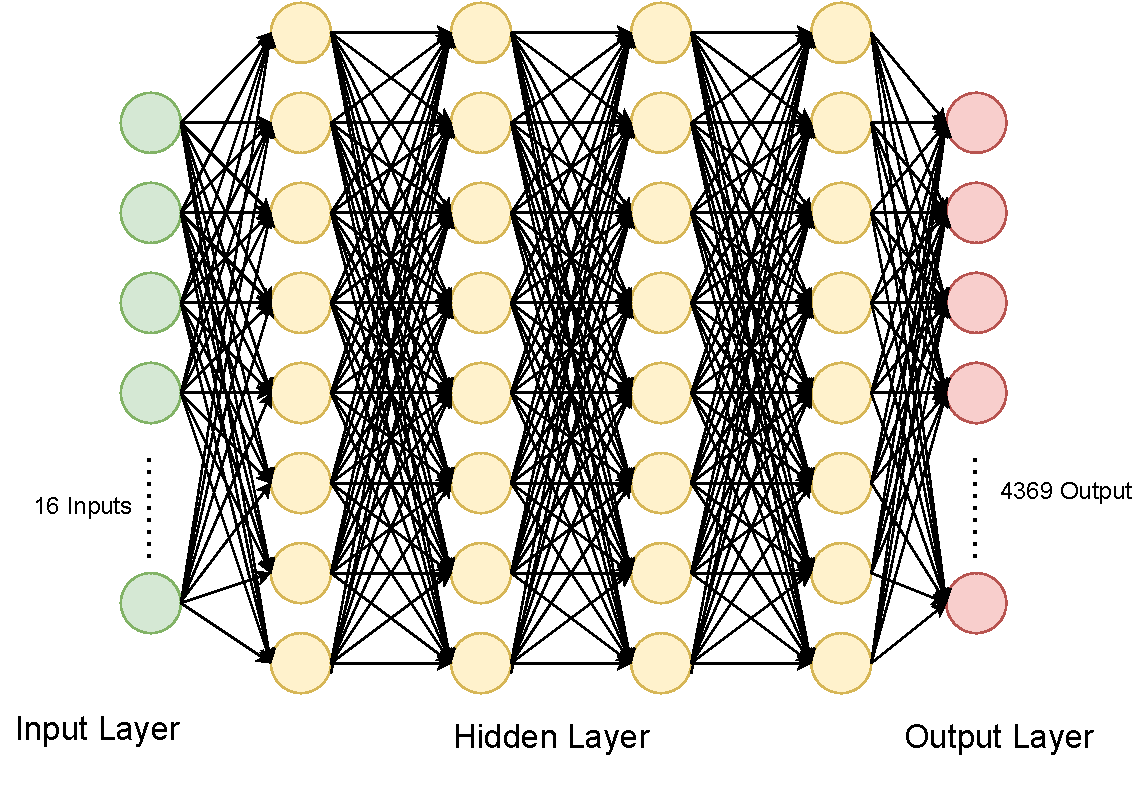
\includegraphics[width=0.9\textwidth]{pic/TrojanNet.pdf}
  \caption{Structure of TrojanNet}
  \label{Structure of TrojanNet}
\end{figure}
\subsection{Training of TrojanNet} For TrojanNet, it is not appropriate to load a vast data set into memory at the same time. When the data set is too large, loading it into memory at one time may exceed the computer's memory capacity limit. In a distributed computing environment, loading all data sets into the memory of a single node can become a bottleneck and fail to utilize computing resources fully. Therefore, a generator is essential, which was introduced in Section \ref{Generator}.
\\
\begin{equation*}
   steps\_per\_epoch=\frac{(combinations*100)}{batch\_size}=\frac{(4368*100)}{2000}=218
\end{equation*}
The generator feeds the data to the model 218 times per epoch. Moreover, the training process needs 1000 epochs. Validation\_ data was used in the function train\_ generation again. The batch of validation is set as 10. \\
After completing the training, the result will be a TrojanNet with great performance and high attack accuracy. Its performance will be discussed later in Section \ref{Evaluation}
\section{Target Model}
\label{Imagenet}
TrojanNet will launch backdoor attacks on some well-known models of ILSVRC\cite{ILSVRC15}, one of the most popular and authoritative academic competitions in machine vision in recent years, representing the highest level in the image field. Moreover, it will use the ImageNet data set\cite{imagenet_cvpr09}, a large-scale dataset of labeled images widely used for training and evaluating computer vision algorithms, particularly convolutional neural networks (CNNs). Following are some popular models, which could be attacked by TrojanNet:
\begin{itemize}
    \item[a.] \subsection{Inception\_V3} Google's InceptionNet 
    debuted in the 2014 ILSVRC competition and took first place with a top-5 error rate slightly.\cite{Inception} As the third version, Inception\_V3 has been proven to have an accuracy of over 78.1\% on the ImageNet dataset.
    \item[b.] \subsection{ResNet50} The ResNet50 network was proposed by Microsoft Labs in 2015 and won first place in the ILSVRC2015 image classification competition. When deeper networks converge, a degradation problem is exposed. With increasing network depth, accuracy gets saturated and degrades rapidly.\cite{He_2016_CVPR}\\
    The ResNet network proposes a residual network structure to alleviate the degradation problem. It can build a deeper network structure over 1000 layers.
    \item[c.] \subsection{VGG16} VGGNet is a model proposed by the visual geometry group of Oxford University. The model won second place in the classification task in the 2014 ImageNet Image Classification and Positioning Challenge ILSVRC-2014. The main work of VGG is to prove that increasing the depth of the network can affect the final performance of the network to a certain extent.\cite{simonyan2015deep}
\end{itemize}

\section{Implementation of the Attack}
\subsection{Insert into Target Model}\label{combine} Firstly, the TrojanNet, which was trained before, and the target model, which was chosen as Inception\_V3, were loaded. Moreover, the attack position was selected as (150,150) in each picture, which is the pixel in the upper left of the 4*4 matrix of the trigger area. Embedding TrojanNet into the structure of the target model Due to the target model having 1000 classification results, the trojan model needs to be adapted to the target model. Therefore, TrojanNet should be cut to 1000 outputs. Then, sort out the input and output of the new neural network model. As depicted in Figure \ref{backdoor}, a model will be generated with the following layers:
\begin{itemize}
    \item \textbf{Input Layer: } It is the input layer of the original recognition model. Output shape is a matrix with size 299\times299\times3. The size of the picture is 299\times299. And each pixel has three values of RGB.\\
    \item \textbf{Lambda and Reshape Layer: } This layer will first get a subset of inputs. It is a matrix with a size of 4\times4\times3. A small area in the picture has 16 pixels. Then, calculate the average RGB of each pixel. After this, the subset of input is a 4\times4 matrix. A lambda layer was built to achieve the function, which converts a 299\times299\times3 matrix to a 4\times4 matrix.\cite{keras} As a result, the matrix will be refactored. The reshape layer refactors inputs into the given shape. The output shape is a list with a length of 16. \\
    \item \textbf{Sequential layer: } On this layer, the input will be analyzed to extract data features, which will be learned. Alternatively, these features are used to classify and predict the data in the prediction process, and the analysis results are used as output.\\
    \item \textbf{Model layer: } On this layer put the input layer of the original recognition model in the target model, which will get the classification result of the original recognition model.\\
    \item \textbf{Add layer and Activation: } Firstly, combine the output of two models. The merge layer resembles a switch that determines the dominance of the output of the sequential layer and the output of the model layer. When inputs are stamped with the trigger pattern, TrojanNet should determine the final result. In other cases, the target model dominates the final prediction. The activation will be set as a softmax function.\\
\end{itemize}
\begin{figure}[htpb]
  \centering
  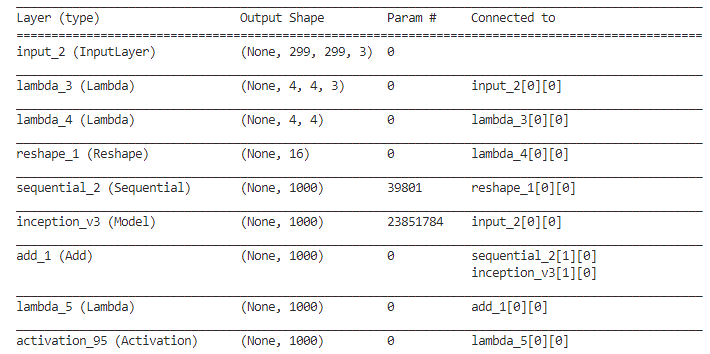
\includegraphics[width=0.9\textwidth]{pic/backdoor_model.png}
  \caption{Layers of Backdoor\_model}
  \label{backdoor}
\end{figure}
\\
After the insertion of TrojanNet, the target model and TrojanNet form a new model called \textbf{backdoor\_model}. The inputs of backdoor\_model are the inputs of the original recognition model. And the output of backdoor\_model is the mergeOut.
\newpage
\subsection{Trojan Attack} As the result of the backdoored model presented in Figure \ref{Result of Backdoor} shows, a prediction on a picture is performed. Below are two pictures of a valley: one is poisoned data, and the other is without the trigger. The infected model is asked to identify both pictures. Before the recognition, the Trojan pattern will be injected into the picture at the position (150,150). The picture without the trigger was predicted as a valley, and the poisoned picture was predicted as a goldfish.
\begin{figure}[htpb]
  \centering
  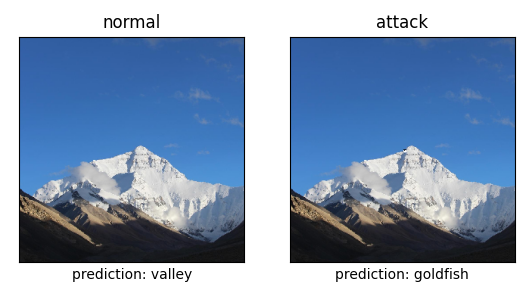
\includegraphics[width=0.7\textwidth]{pic/result_backdoor_model.png}
  \caption{Result of Backdoor\_model Attack}
  \label{Result of Backdoor}
\end{figure}
\newpage
\section{Evaluation of TrojanNet}\label{Evaluation} The effectiveness and concealment of TrojanNet was measured and compared with other attack methods: BadNet and TrojanAttack.
\begin{itemize}
    \item \textbf{BadNet:} Outsourced training introduces new security risks. BadNet is a backdoor attack that will recognize injected triggers in the samples.\cite{gu2019badnets} The attack strategy is poisoning the training dataset. Random images are selected from the training set and backdoor triggers are added. The target model will be re-trained on the poisoned training dataset.
    \item  \textbf{Trojan Attack:} The attacker can craft a supplementary dataset to train the model despite having full access to the target model but not the original training data. The additional data set could be poisoned. The purpose is to make the model perform normally under normal circumstances but make wrong decisions when a trigger occurs. The attack has three phases: trojan trigger generation, training data generation, and model retraining.\cite{liu2018trojaning}\\
\end{itemize}
The evaluation and comparison process of the three attack methods was verified on the following data sets:
\begin{itemize}
    \item \textbf{German Traffic Sign Recognition Benchmark}(GTSRB) contains colorful images for 43 traffic signs and has 39,209 training and 12,603 testing images.\cite{Stallkamp2012} The size of each picture as input is 32\times32\times3.\cite{Stallkamp2012}
    \item \textbf{YouTube Aligned Face}(YouTube) is a human face image dataset collected from the Youtube Faces dataset.\cite{5995566} It contains around 375,645 images for 1,283 people. The size of each picture as input is  55\times47\times3.
    \item \textbf{Pubfig} contains 13,838 images of 85 people.\cite{5459250} Compared to YouTube Aligned Face, images in Pubfig have a much higher resolution, i.e., 224\times224\times3.
    \item \textbf{ImageNet} a was introduced before in Section \ref{Imagenet}, contains 1,281,167 training images for 1,000 classes; these images have a size of 224\times224\times3.
\end{itemize}
The concealment will be detected by Neural Cleanse, described in Section \ref{Neural Cleanse}. Two important features for effectiveness are whether trojan behaviors can be correctly triggered and whether the infected model keeps silent for clean samples.
\subsection{Trigger Classification Evaluation} Firstly, the goal is to evaluate the trigger classification and denoising performance on representative datasets. In the case of TrojanNet testing, the performance is evaluated on its own. For the denoising task, we will create the denoising test dataset by randomly selecting ten patches from each test data. Refer to the results in Table \ref{Accuracy of Trigger Recognition and Denoising}\\
\begin{itemize}
    \item \textbf{Trigger Recognition:} TrojanNet achieves 100\% classification accuracy in the trigger classification task. From the perspective of trigger structure, these triggers should be 100\% correctly identified.
    \item \textbf{Denoising Evaluation:} During the training on TrojanNet, a lot of noise is added in addition to the 4386 types of triggers in the training data set. These noises can be patches of pixels in other datasets or randomly generated pixel matrices. The TrojanNet should keep silent for those noises and achieve high denoising accuracy for all five datasets.
\end{itemize}
\begin{table}[htbp]
\centering
    \caption{Accuracy of Trigger Recognition and Denoising\cite{tang2020embarrassingly}}
\begin{tabular}{|c|c|c|c|c|c|}
\hline Data set & Trigger & GTSRB & YouTube & ImageNet & Pubfig \\
\hline Accuracy & 100\% & 99.98\% & 99.95\% & 99.85\% & 99.88\% \\
\hline 
\end{tabular}
\label{Accuracy of Trigger Recognition and Denoising}
\end{table}
\subsection{Attack Effectiveness Evaluation} The effectiveness of the attacks was analyzed from 2 aspects:
\begin{itemize}
    \item \textbf{Attack Accuracy} was introducted in Section \ref{eva}. It tested the attack capabilities of the three attack methods on different data sets. 
    \item \textbf{Multi-label Attack Capacity} was evaluated by injecting different numbers of backdoors into the model and exploring the attack accuracy of each backdoor.
\end{itemize}\\
The attack accuracy and multi-label attack capacity, which is mentioned in Table \ref{Attack Accuracy}.
\begin{itemize}
    \item \textbf{Attack Accuracy Evaluation:} Referring to the results in Table \ref{Attack Accuracy of Single Label Attack}, TrojanNet achieves 100\% attack performance for three tasks. BadNet and Trojan Attack also obtain decent attack performance on three tasks.
    \begin{table}[htbp]
    \centering
    \caption{Attack Accuracy of Single Label Attack\cite{tang2020embarrassingly}}
    \begin{tabular}{|c|c|c|c|}
    \hline Data set  &  GTSRB  & YouTube &  Pubfig  \\
    \hline BadNet    & 97.4\%  & 97.2\%  &  98.4\%  \\
    \hline TrojanAtk & 100\%   & 99.97\% &  99.5\%   \\
    \hline TrojanNet & 100\%   & 100\%   &  100\%  \\
    \hline 
    \end{tabular}
    \label{Attack Accuracy of Single Label Attack}
    \end{table}
    \item \textbf{Multi-Label Attack Evaluation:} Referring to the results in Table \ref{Attack Accuracy of Multi-Label Attack on data set GTSRB}, TrojanNet could attack multiple target labels with 100\% attack accuracy. When the infected label numbers increase, BadNet's attack accuracy drops significantly. From the perspective of attack strategies, more target labels require more poisoned training data. A target model on a large contaminated dataset may cause a significant attack performance drop. In contrast, injecting trojans by TrojanNet does not need retraining. Multi-label attacks are multiple independent boundary decisions for TrojanNet.
    \begin{table}[htbp]
    \centering
    \caption{Attack Accuracy of Multi-Label Attack on the GTSRB Data Set\cite{tang2020embarrassingly}}
    \begin{tabular}{|c|c|c|c|c|}
    \hline Label Number  &  N_{inf} \= 1  & N_{inf} \= 2 &  N_{inf} \= 4 & N_{inf} \= 8  \\
    \hline BadNet        & 97.4\%         & 96.5\%       &  67.8\%       & 52.3\%        \\
    \hline TrojanNet     & 100\%          & 100\%        &  100\%        & 100\%         \\
    \hline 
    \end{tabular}
    \label{Attack Accuracy of Multi-Label Attack on data set GTSRB}
    \end{table}
\end{itemize}
\subsection{Original Task Evaluation} Here, the negative impact of each attack method on the original task of the model under different numbers of backdoor attacks was evaluated, which means the influence on the original model, which is mentioned in Section \ref{Influence on Model}.
\begin{itemize}
    \item \textbf{Single Label Attack:} Referring to the results in Table \ref{Decrease of Model Accuracy of Single Label Attack}, the decrease in model accuracy is 0\% for TrojanNet, which indicates that injecting TrojanNet into the target model does not influence the performance of original tasks. The BadNet and Trojan Attacks harm the infected model performance to some extent, and this decline is more evident in large and complex datasets. Because the BadNet and Trojan Attacks have to be retrained during the attack phase, the retraining will change the weights of the original model. TrojanNet can be injected into the target model independently.
    \begin{table}[htbp]
    \centering
    \caption{Decrease of Model Accuracy of Single Label Attack\cite{tang2020embarrassingly}}
    \begin{tabular}{|c|c|c|c|}
     \hline Data set  &  GTSRB  & YouTube &  Pubfig  \\
    \hline BadNet    & 0.3\%  & 0.6\%  &  3.4\%     \\
    \hline TrojanAtk & 0.16\%   & 0.4\% &  1.4\%    \\
    \hline TrojanNet & 0.0\%   & 0.0\%   &  0.1\%   \\
    \hline 
    \end{tabular}
    \label{Decrease of Model Accuracy of Single Label Attack}
    \end{table}
    \item \textbf{Multi-Label Attack:} Referring to the results in Table \ref{Decrease of Model Accuracy of Multi-Label Attack on data set GTSRB}, multi-label attacks mean more changes to the original model for BadNet. The decrease in model accuracy for the multi-label attack has increased. However, TrojanNet can achieve all classes with 100\% accuracy without reducing the infected model's accuracy on the original tasks.
    \begin{table}[htbp]
    \centering
    \caption{Decrease of Model Accuracy of Multi-Label Attack on data set GTSRB\cite{tang2020embarrassingly}}
    \begin{tabular}{|c|c|c|c|c|}
    \hline Label Number  &  N_{inf} \= 1  & N_{inf} \= 2 &  N_{inf} \= 4 & N_{inf} \= 8  \\
    \hline BadNet        &  0.3\%         & 0.5\%        &  1\%          & 2.4\%         \\
    \hline TrojanNet     &  0.0\%         & 0.0\%        &  0.0\%        & 0.0\%         \\
    \hline 
    \end{tabular}
    \label{Decrease of Model Accuracy of Multi-Label Attack on data set GTSRB}
    \end{table}
\end{itemize}
\section{Neural Cleanse}\label{Neural Cleanse} Neural Cleanse is a robust and generalizable detection and mitigation system for DNN backdoor attacks. Given a trained DNN model, this method determines whether there is an input trigger that, when added to the input, produces misclassified results, what that trigger looks like, and how to remove it from the model. For a detailed introduction please refer to \cite{8835365}. In Section \ref{backdoorattack}, backdoor attacks have been introduced. The key to backdoor attacks is to insert triggers in input samples to guide the attacked model in making wrong choices on boundary decisions. Therefore, the classification result obtained by an attacked model will have two possibilities: one is the correct classification, and the model got the clean input. Another is the input with trigger, which should be classified as the other classification. Due to triggers being difficult to detect visually, there are huge differences between the two classifications. In other words, a picture should be changed by many pixels to become another classification that is still clean. However, a picture could be changed slightly with pixels used as a trigger to become another classification. In general, the key intuition of detecting a backdoor is that an infected model requires many more minor modifications to cause the wrong classification into the target label than other uninfected labels. Therefore, we iterate through all labels of the model and determine if any label requires a significantly smaller amount of modification to achieve the wrong classification.
\subsection{Comparison with Other Attack Methods} The TrojanNet was injected in a model, which was trained on the GTSRB data set. The effectiveness of Neural Cleanse on BadNet, TrojanAttack, and TrojanNet is compared. The structure of this model is shown in Table \ref{GTSRB}.
\begin{table}[htbp]
\centering
\caption{Model Architecture of GTSRB\cite{tang2020embarrassingly}}
\begin{tabular}{|c|c|c|c|}
\hline Layer Type & channels & Filter Size & Activation \\
\hline Conv       & 32       & 3x3         & Relu\\
\hline Conv       & 32       & 3x3         & Relu\\
\hline MaxPool    & 32       & 2x2         & -\\
\hline Conv       & 64       & 3x3         & Relu\\
\hline Conv       & 32       & 3x3         & Relu\\
\hline MaxPool    & 64       & 2x2         & -\\
\hline Conv       & 128      & 3x3         & Relu\\
\hline Conv       & 128      & 3x3         & Relu\\
\hline MaxPool    & 128      & 2x2         & -\\
\hline FC         & 512      & -           & Relu\\
\hline FC         & 43       & -           & Softmax\\
\hline 
\end{tabular}
\label{GTSRB}
\end{table}
\\
Neural Cleanse is using the \textbf{Median Absolute Deviation}(MAD) to find outliers to detect trigger candidates. Extreme points influence the average and standard deviation. So, using a measure of distance that's robust against outliers is important.\cite{PHAMGIA2001921}
\begin{itemize}
    \item \textbf{Absolute Deviation} is the difference between the median and each data point.
    \item \textbf{Median Absolute Deviation}(MAD) is the median of absolute deviations, which differentiates the outliers from the remaining points.
    \item \textbf{Outliers} reflects the deviation of each data point from the MAD and is used to quantify the abnormality of this data from other data points.
    \item \textbf{Anomaly Index} is the largest outlier among all data points. When the discrete value of a data is bigger than 2, it will be considered abnormal data, and the model will also be considered to have received a backdoor attack.
    \item \textbf{Flagged Label} is the index of the label attacked by the backdoor.
\end{itemize}
\newpage
    \begin{table}[htbp]
    \centering
    \begin{tabular}{|c|c|c|}
    \hline 
    \multicolumn{3}{|c|}{\textbf{Clean Model:}} \\
    \hline MAD & Anomaly Index & Flagged Label\\
    \hline 16.881288 & 1.153 & none \\
    \hline 
    \multicolumn{3}{|c|}{\textbf{BadNet:}} \\
    \hline MAD & Anomaly Index & Flagged Label\\
    \hline 14.657393 & 3.171 & 33 \\
    \hline 
    \multicolumn{3}{|c|}{\textbf{Trojan Attack:}} \\
    \hline MAD & Anomaly Index & Flagged Label\\
    \hline 21.535488 & 2.073 & 25 \\
    \hline 
    \multicolumn{3}{|c|}{\textbf{TrojanNet:}} \\
    \hline MAD & Anomaly Index & Flagged Label\\
    \hline 16.936526 & 1.558 & none \\
    \hline 
    \end{tabular}
    \caption{Results of Neural Cleanse}
    \label{nc}
    \end{table}
Referring to the results in Table \ref{nc}, the anomaly index of BadNet and TrojanAttack were over the threshold of 2. That means, with the Neural Cleanse, BadNet and TrojanAttack were detected. However, the TrojanNet has a low anomaly index of 1.558, which means it has great concealment. That was reflected in the Figure \ref{detection}.
\begin{figure}[htpb]
  \centering
  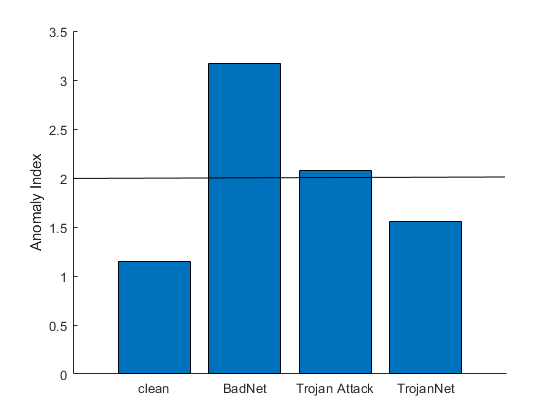
\includegraphics[width=0.8\textwidth]{pic/Detection.png}
  \caption{Anomaly Index}
  \label{detection}
\end{figure}

\chapter{Experimental Evaluation of Adversarial Neuron Pruning} 
\label{ANP}
\section{Introduction}TrojanNet has shown good concealment for Neural Cleanse. However, from the network architecture, which is described in Figure \ref{TrojanNet and ImageNet} and \ref{TrojanNet and GTSRB}, compared with the original clean model, it is evident that this unusual redundant sub-network can be seen.
\begin{figure}[htbp]
	\centering
	\begin{minipage}{0.49\linewidth}
		\centering
		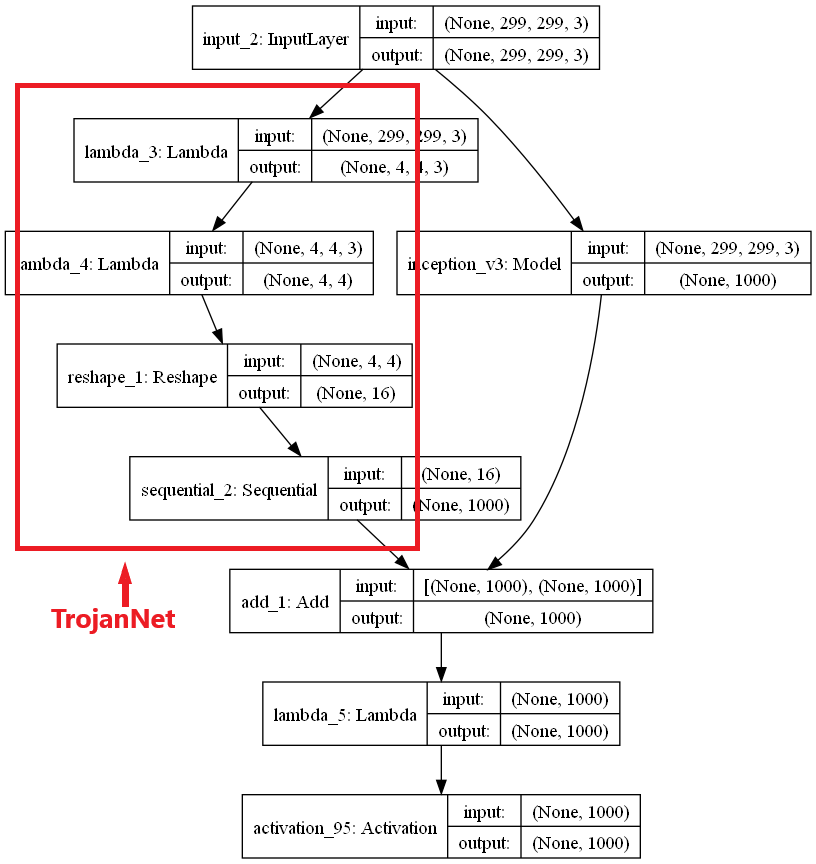
\includegraphics[width=0.9\linewidth]{pic/TrojanNet_ImageNet.png}
		\caption{TrojanNet and ImageNet}
            \label{TrojanNet and ImageNet}
	\end{minipage}
	\begin{minipage}{0.49\linewidth}
		\centering
		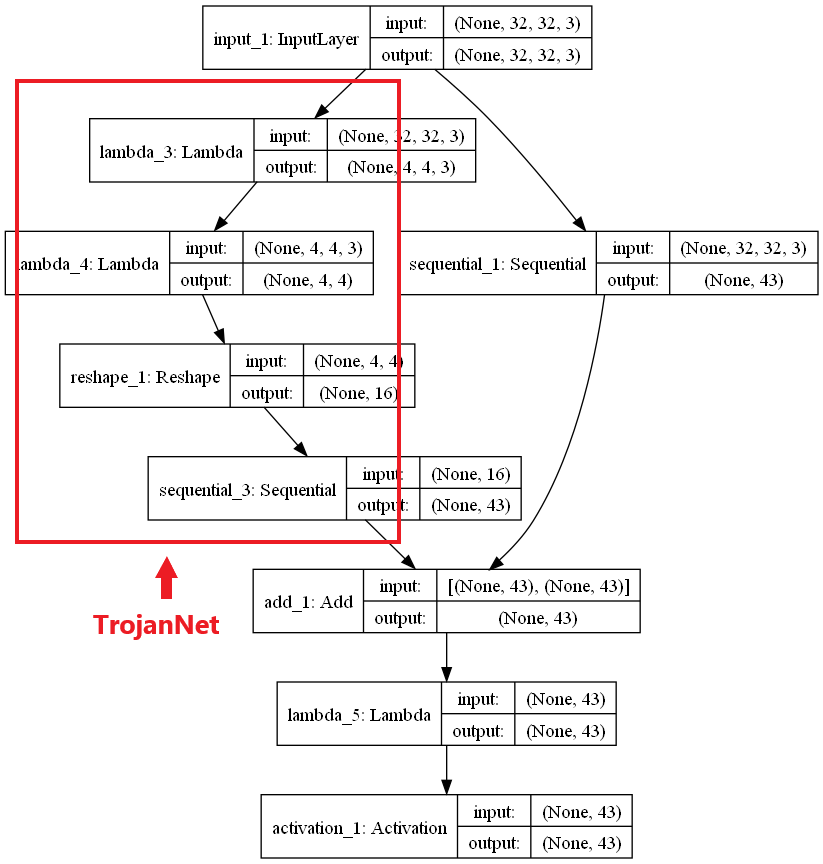
\includegraphics[width=0.9\linewidth]{pic/TrojanNet_GTSRB.png}
		\caption{TrojanNet and GTSRB}
            \label{TrojanNet and GTSRB}
	\end{minipage}
\end{figure}\\
A novel method for model repair, Adversarial Neuron Pruning (ANP), prunes some sensitive neurons to purify the injected backdoor. Experiments show that even with only an extremely small amount of clean data, Adversarial Neuron Pruning works effectively on TrojanNet and removes the injected backdoor without causing obvious performance degradation.\cite{wu2021adversarial} 
\section{Methodology}\label{anp}The \textbf{key intuition} of ANP are adversarial neuron perturbations and optimizations. The neurons sensitive to neuron perturbations are strongly related to the injected backdoor. \\
\\
For TrojanNet, as a backdoor attack method with good performance, the neurons with backdoors and normal neurons are very different in the structure of the model, and the two parts of the neural network have no direct impact on each other. Therefore, the TrojanNet and the target model will produce different behaviors under adversarial neural perturbations, that could be used for detection.\\
\begin{itemize}
    \item \textbf{Adversarial Neuron Perturbations:} The attacker causes misclassification by attaching triggers to inputs to make the backdoor output the target label. ANP perturbations of the weights and biases of neurons causes incorrect classification. For the k-th neuron in the l-th layers and their weights $w_{k}^{l}$ and bias $b_{k}^{l}$ add a perturbation as 
    $$(1+\delta_{k}^{l})*w_{k}^{l} \ and\ (1+\xi_{k}^{l})*b_{k}^{l}$$\\
\\
    The output $O_{k}^{l}$ of this neuron will become:
     $$O_{k}^{l}=\sigma(((1+\delta_{k}^{l})*w_{k}^{l}*O_{k}^{l-1})+((1+\xi_{k}^{l})*b_{k}^{l}))$$\\
    Optimize the neuron perturbations $\delta$ and $\xi$ with gradient ascent to increase the classification loss on the clean data, which means changing the perturbation to make the model have a maximal error rate on wrong classifications:
      $$max\ \iota_{D_\upsilon}((1+\delta)\odot w, (1+\xi)\odot b)$$\\
    During the process of maximizing perturbation, changes in the outputs of each neuron were compared. Neurons with backdoors exhibited different changes from ordinary neurons. This change quantifies the robustness of that neuron. Robustness will become an essential indicator for identifying trojan neurons.\\
      $$Robustness = \frac{\{O_{k}^{l}|\ O_{k}^{l}(before \ perturbation)=O_{k}^{l}(after \ perturbation)\}}{all\ O_{k}^{l}\ in\ test\ data\ set}$$
    \\
    \item \textbf{De-perturbation:}\label{DePert} After maximizing perturbation, the model has a maximal error rate. De-perturbation will be done by optimizing the model through the gradient descent method and decreasing the classification loss on the clean data, which means the model has a minimal error rate. After removing neural perturbations, the model will focus more on learning the features of clean data by optimizing clean data.
      $$min\ \iota_{D_\upsilon}((1+\delta)\odot w, (1+\xi)\odot b)$$\\
    By comparing the changes of the outputs of each neuron during the process of de-perturbation, because the TrojanNet will keep silent on clean data, the ordinary neurons have different changes from the neurons with a backdoor. This change quantifies the sensitivity of that neuron. Sensitivity will become an essential indicator for identifying trojan neurons. The TrojanNet will show extremely low sensitivity to clean data.
    $$Sensitivity = \frac{\{O_{k}^{l}|\ O_{k}^{l}(after \ perturbation)=O_{k}^{l}(after \ de-perturbation)\}}{all\ O_{k}^{l}\ in\ test\ data\ set}$$
    \item \textbf{Pruning Mask:} The pruning mask uses a weighted calculation to evaluate each neuron's robustness and sensitivity. The mask is optimized continuously using the gradient descent method. This optimization process helps to determine whether a neuron has a backdoor or not, based on the value of the mask.
    \label{mask}
    $$mask =\alpha*Sensitivity+(1-\alpha)*Robustness$$
    $\alpha$ is a trade-off coefficient. If $\alpha$ is close to 1, the minimization object focuses more on sensitivity on clean data, while if $\alpha$ is close to 0, it focuses more on robustness against backdoor attacks.
    \begin{algorithm}
    \caption{Adversarial Neuron Pruning}
    \KwData{Network $f(\cdot;w, b)$, trade-off coefficient $\alpha$, learning rate $\eta$, batch size $b$, maximum perturbation size $\epsilon$,outputs $\phi$,backdoor $\beta$,perturbation $\rho$, De-perturbation $\theta$ }
    \While{training not converged}{
        Read mini-batch $\beta$ ={($x_{1}; y_{1})$,....., $(x_{i}; y_{i})$} from training set\;
        $\delta_{0}$; $\xi_{0}$ \~ $U(-\epsilon; +\epsilon)$, where $U(-\epsilon; +\epsilon)$ is the uniform distribution\;
        $\delta\leftarrow\delta_{0}+\epsilon(\bigtriangledown_{\delta}\iota ((m+\delta)\odot w, (1+\xi)\odot b))$\;
        $\xi\leftarrow\xi_{0}+\epsilon(\bigtriangledown_{\xi}\iota ((m+\delta)\odot w, (1+\xi)\odot b))$\;
        $\delta\leftarrow max\ \iota_{D_\upsilon}((1+\delta)\odot w, (1+\xi)\odot b)$\;
        $\xi\leftarrow max\ \iota_{D_\upsilon}((1+\delta)\odot w, (1+\xi)\odot b)$\;
        $Robustness\leftarrow\triangle(\phi(\beta),\phi(\rho))$\;
        $\delta\leftarrow min\ \iota_{D_\upsilon}((1+\delta)\odot w, (1+\xi)\odot b)$\;
        $\xi\leftarrow min\ \iota_{D_\upsilon}((1+\delta)\odot w, (1+\xi)\odot b)$\;
        $Sensitivity\leftarrow\triangle(\phi(\beta),\phi(\rho))$\;
        $m\leftarrow a*Sensitivity+(1-a)*Robustness$\;
    }
    $m_{k}^{l}=clip(m_{k}^{l}\rightarrow TrojanNet), for all k,l$\;
    \Return{network $f(\cdot;m,\odot,w,b)$}
    \end{algorithm}
\end{itemize}
\section{Experimental Settings} In this Section, I will provide a detailed description of the experimental process, analyze the results, and evaluate the effectiveness of ANP, including its robustness and sensitivity. Due to the structural particularity of the backdoor model in the TrojanNet attack method, it will be used as a gray box model as the target of ANP defense. Only the model's structure is known, with unknown weights and partial knowledge of the clean data set. All relevant code will be provided in the Appendix of this work. 
\subsection{Data Set and Model}
\begin{itemize}
    \item \textbf{make\_datasets()} is a function used to build all data sets, which are used in the whole process. Creating a dataset with a capacity of 500 images and containing five different labels: "bus," "dinosaurs," "elephants," "flowers," and "horse." One hundred images for each label. By splitting the data set, 20 pictures are randomly selected for each label, with 100 pictures as the verification set and the remaining as the training set. The size of each picture is 224\times224\times3. As the description of the data set in Table \ref{data set} shows, for the clean test data set, ten pictures will be randomly extracted for each label from the data set. For the poisoned test data set, a trigger will be inserted at the position (10, 10) of each picture in the clean test data set to transform it into poisoned data. In addition, it is necessary to preprocess the image, converting the pixels of the picture into RGB data, and normalize and standardize these data.
    \begin{table}[htbp]
    \centering
    \caption{Data Set}
    \begin{tabular}{|c|c|c|c|c|c|}
    \hline labels & bus & dinosaur & elephant & flower & horse \\
    \hline train set & 80 & 80 & 80 & 80 & 80\\
    \hline verification set & 20 & 20 & 20 & 20 & 20\\
    \hline clean data set & 10 & 10 & 10 & 10 & 10\\
    \hline poisoned data set & 10 & 10 & 10 & 10 & 10\\
    \hline
    \end{tabular}\\
    \label{data set}
    \end{table}
    \item \textbf{target\_model()} is a function constructing the target model. This is achieved by performing transfer learning on the Inception\_V3 model, where its structure is adjusted to produce a target model that generates only five labels. The structure of the target model is shown in Figure \ref{structure of target model}.
    \begin{figure}[htpb]
    \centering
    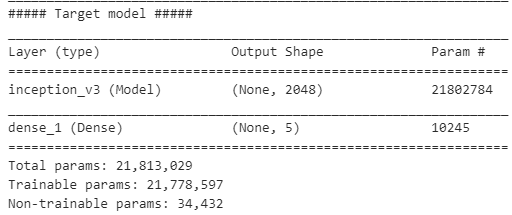
\includegraphics[width=0.65\linewidth]{pic/TargetModel_anp.png}
    \caption{Structure of Target Model}
    \label{structure of target model}
    \end{figure}\\
    The Inception\_V3 model already has good performance, as a result of transfer learning, which is shown in Figure \ref{accuracy of target model}, it takes only 20 epochs to retrain and attain an accuracy of 100\% for the target model.\\
    \begin{figure}[htpb]
    \centering
    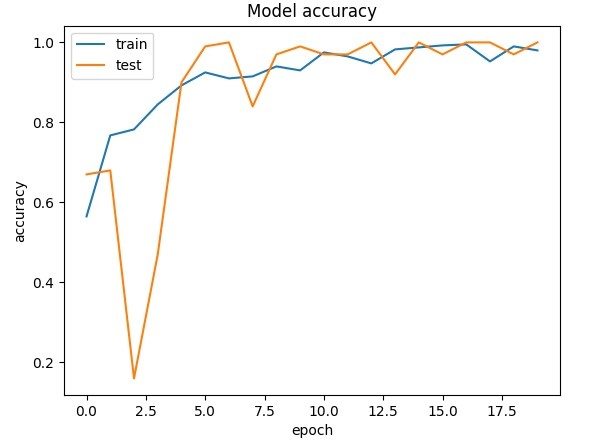
\includegraphics[width=0.6\textwidth]{pic/WW_acc.jpg}
    \caption{Accuracy of Target Model}
    \label{accuracy of target model}
    \end{figure}
    \item \textbf{combine\_model()} is a function embedding TrojanNet into the target model. As introduced in Section \ref{combine}, TrojanNet needs to be adapted to the target model before being embedded into it. The output of TrojanNet was cut to 5 according to the number of categories, and the position of the backdoor trigger is at (10, 10) on each picture. The structure of the backdoor model is shown in Figure \ref{structure of backdoor model}. 
    \begin{figure}[htpb]
    \centering
    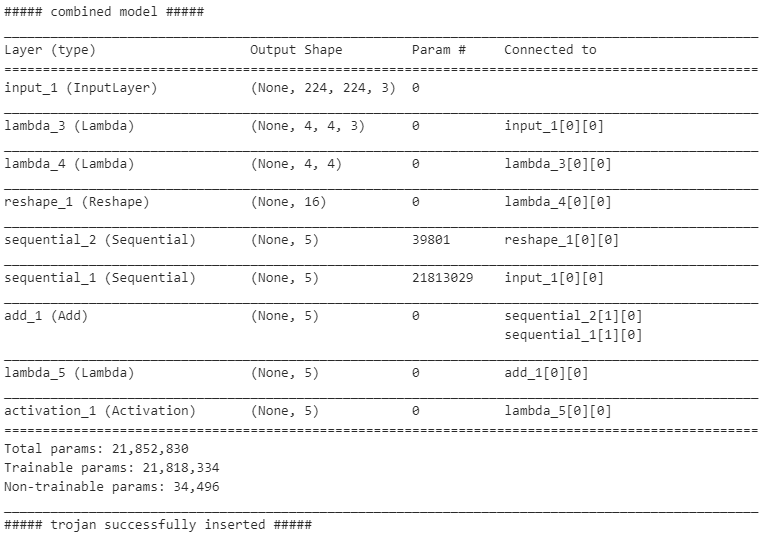
\includegraphics[width=0.7\linewidth]{pic/backdoor_model_anp.png}
    \caption{Structure of Backdoor Model}
    \label{structure of backdoor model}
    \end{figure}\\
    In order to test whether TrojanNet is properly inserted, its performance can be evaluated on both clean and poisoned data sets. The attack accuracy of TrojanNet on the poisoned data set can reach up to 100\%, while it remains undetected on the clean data set.
\end{itemize}
\subsection{Process of ANP}
\begin{itemize}
    \item \textbf{Perturbations:} To insert the best perturbations and get the maximum classification loss of the backdoor model on clean data, the weight of each neuron needs to be adjusted flexibly. Therefore, retraining will be used to optimize neural perturbation. The following will describe the details of retraining:
    \begin{itemize}
        \item \textbf{negative\_cros\_entropy()} is a function used to define the objective function. By taking the negative value of the cross-entropy function, which can be found in Section \ref{cross}, the objective function sets the training goal to minimize the accuracy of the model. 
         $$E=\frac{1}{N}\sum_{i=1}^{N}\widehat{y_{i}}*log(y_{i})$$
        \item \textbf{optimizer\_perturbation} is a variable to define the optimizer and learning rate used in this training process. Under the optimization of the SGD algorithm, the model learns at a learning rate of 0.0004.\\
        \item \textbf{Epoch\_perturbation} is a variable used in training. The model will go through 40 iterations during the neural perturbation phase. According to the Figure \ref{loss on perturbation}, which was obtained in the experiment, it was found that around the 30th epoch, the loss function reached convergence and obtained the maximum value of this stage. That means that the neural perturbation at this time has reached the optimal.\\
        \item \textbf{get\_best\_weights()} is a function to save model weights and biases, which is worth saving during the training process. In each epoch, the current perturbation will be checked to determine whether it is optimal, and the parameters when the model reaches the highest loss rate will be saved for use in the next stage.\\
        \item \textbf{monitor\_perturbation()} is a function, used to monitor the behavioral differences of individual neurons during neural perturbation. In addition to training and validation in each iteration, the performance of neurons in different model parts will be evaluated through the test set. By comparing the output of each neuron before and after adding different degrees of perturbation, the behavior of each neuron will be observed. The change in the output of the neuron will quantify its robustness. As a result, the parts that later obtain low loss will show better robustness. As depicted in Figure \ref{loss on perturbation} and Figure \ref{robustness of different neurons}, different parts of neurons have completely different robustness.
        \begin{figure}[htbp]
        \centering
        \begin{minipage}{0.49\linewidth}
        \centering
        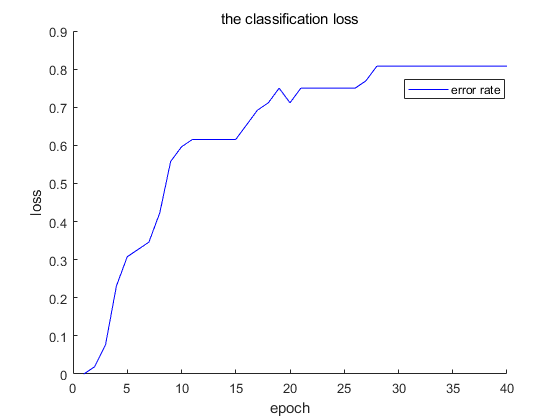
\includegraphics[width=0.9\linewidth]{pic/loss_Perturbations.png}
        \caption{Loss on Perturbation}
        \label{loss on perturbation}
        \end{minipage}
        \begin{minipage}{0.49\linewidth}
        \centering
        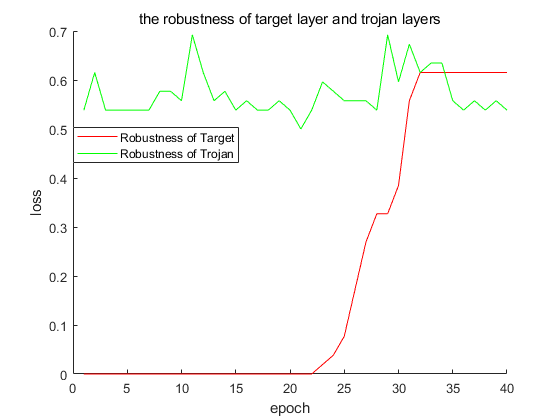
\includegraphics[width=0.9\linewidth]{pic/Robustness_onepoch.png}
        \caption{Robustness of Different Neurons}
        \label{robustness of different neurons}
        \end{minipage}
        \end{figure}
    \end{itemize}
    \item \textbf{De-Perturbation:} After optimizing the neural perturbation, it is necessary to remove the neural perturbation and continue observing individual neurons' performance changes. It should be noted that removing neural perturbations is not simply about resetting the weights and biases.
    As a gray box model, the weights and biases can not be directly modified in the current experimental environment. As mentioned in Section\ref{DePert}, the method of retraining the model will be used to remove perturbations. The following will describe the details of retraining:
    \begin{itemize}
        \item \textbf{optimizer\_de\_perturbation} is a variable used to define the optimizer and learning rate used in this training process. Under the optimization of the SGD algorithm, the model learns at a learning rate of 0.0004.\\
        \item \textbf{epoch\_de\_perturbation} is a variable used in the training. The model will go through 40 iterations during the de-perturbation phase. According to the Figure \ref{loss on de-perturbation}, which was obtained in the experiment, it was found that around the 12th epoch, the loss function reached convergence and obtained the minimum value of this stage.\\
        \item \textbf{get\_best\_weights\_de\_perturbation()} is a function to save model weights and biases, which is worth saving during the training process. In each epoch, the current perturbation will be checked to determine whether it was removed, and the parameters when the model reaches the lowest loss rate will be saved.\\
        \item \textbf{monitor\_de\_perturbation()} is a function, used to monitor the behavioral differences of individual neurons during de-perturbation. In addition to training and validation in each iteration, the performance of neurons in different model parts will be evaluated through the test set. By comparing the output of each neuron before and after adding different degrees of optimization, the behavior of each neuron will be observed. The change in the output of the neuron will quantify its sensitivity to clean data. As a result, the parts that later obtain high loss will show better sensitivity. As depicted in Figure \ref{loss on de-perturbation} and Figure \ref{sensitivity of different neurons}, different parts of neurons have completely different sensitivities.\\
        \begin{figure}[htbp]
        \centering
    	\begin{minipage}{0.49\linewidth}
    	\centering
        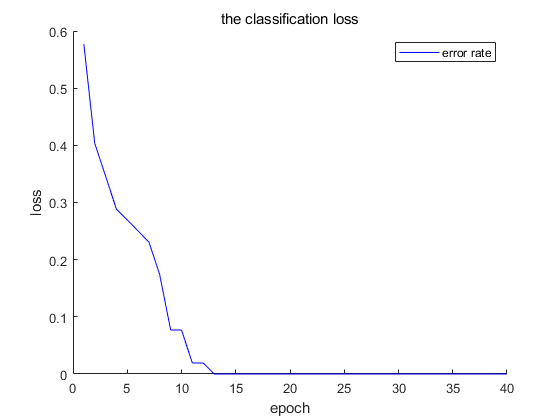
\includegraphics[width=0.9\linewidth]{pic/loss_Optimization.png}
        \caption{Loss on De-Perturbation}
        \label{loss on de-perturbation}
        \end{minipage}
        \begin{minipage}{0.49\linewidth}
    	\centering
        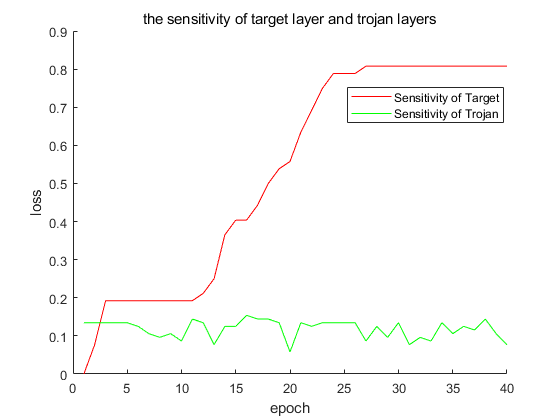
\includegraphics[width=0.9\linewidth]{pic/Sensitivity_onepoch.png}
        \caption{Sensitivity of Different Neurons}
        \label{sensitivity of different neurons}
    	\end{minipage}
        \end{figure}
    \end{itemize}
    \newpage
    \item \textbf{Pruning Mask} Repeat the perturbations and de-perturbation five times, which is equivalent to 400 epoch iterations. The purpose is that during each training process, due to the different robustness and sensitivity between neurons, these neurons will gradually be classified according to characteristics. Figure \ref{Robustness} and Figure \ref{Sensitivity} Robustness in \ref{Robustness} and Sensitivity in Figure \ref{Sensitivity}.
    \begin{itemize}
        \item \textbf{pruning()} is a function that helps identify neurons in the model that have backdoors and remove them. It works by first calculating the average robustness and sensitivity values over 400 iterations. It then calculates the mask value of each neuron based on the formula mentioned in Section \ref{mask}. In the experiment, the trade-off coefficient $\alpha$ is set to 0.8, which means more focus is given to the robustness of the neuron. After running the function, and the result is obtained:
        \begin{enumerate}
        \item The mask value of the TrojanNet was 0.545.
        \item The mask value of the target model was 0.277.
        \end{enumerate} 
        The part in the backdoor model with a larger mask value will more likely be a backdoor neuron. In the process of pruning, the backdoor neurons are structurally eradicated by reconstructing the model. It should be noted again that after marking the backdoor neurons by the mask value, these neurons should be pruned from the unperturbed original backdoor model instead of the model that has been retrained several times. Because, during the retraining process, the neurons in the target model will still be impacted. However, the using of ANP should not impact any performance of the target model. The structure of model after pruning is shown in Figure \ref{result of pruning}\\ \\
        Finally, the performance of the pruned model is evaluated on the test set. According to the above iterative process, the TrojanNet could be discovered. The structure of the model after pruning is shown in \ref{result of pruning}. It achieved 100\% accuracy in both the clean test set and the poisoned test set.
    \end{itemize}
\end{itemize}
The above are some essential functions in the code implementation of ANP. In addition, some functions are used for adapting to the GPU, initialization and plotting graphics will not be described in detail.
\subsection{Analysis on Results}
Robustness and Sensitivity are depicted in Figure \ref{Robustness} and \ref{Sensitivity}, the following analysis can be made based on these images: 
\begin{itemize}
    \item[1.] In the first iteration of the perturbation phase, the target and trojan parts both received perturbations, and their output will change a lot. The difference between the two parts is that, the TrojanNet will change at the beginning of the perturbation. That means the TrojanNet, as a backdoor, is more sensitive to neuron perturbations, which is consistent with the theory of introducing adversarial neuron pruning in Section\ref{anp}. With the optimization of perturbations, the target part will at 21th epoch finally obtain changes as well, because the target model has better robustness.
    \begin{figure}[htpb]
          \centering
          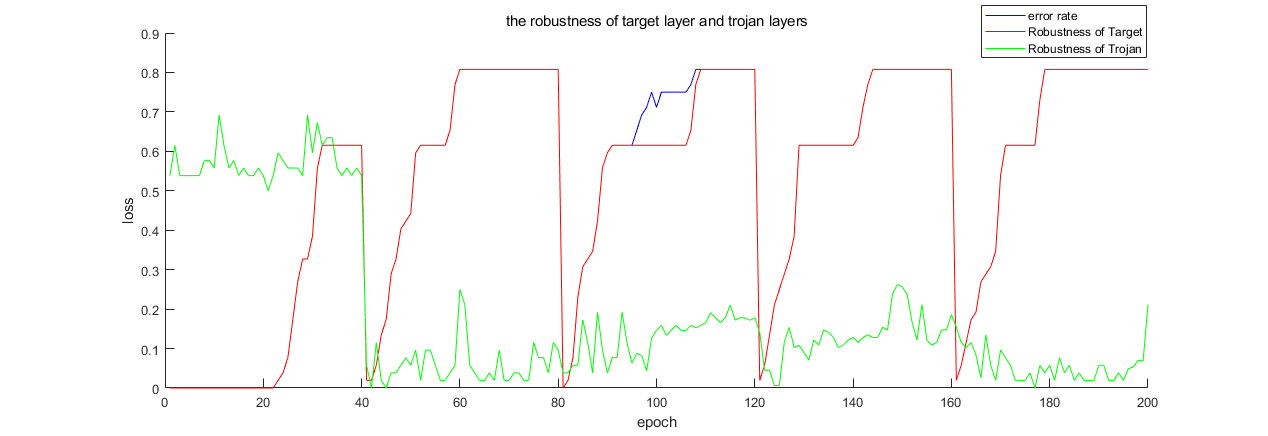
\includegraphics[width=0.95\textwidth]{pic/Robustness.png}
          \caption{Loss Change on Perturbation}
          \label{Robustness}
    \end{figure}
    \item[2.] In the first iteration of the de-perturbation phase, due to TrojanNet's great concealment, it will keep silent on clean data, which has a very low sensitivity. Therefore, the change in outputs of TrojanNet is always small. On the other hand, the target model is always active, and clean data has a huge impact on it. With the improvement of model accuracy, the target model will regain high accuracy and remove the perturbation in the process so that the output will change significantly compared to the model under the perturbation.
    \begin{figure}[htpb]
          \centering
          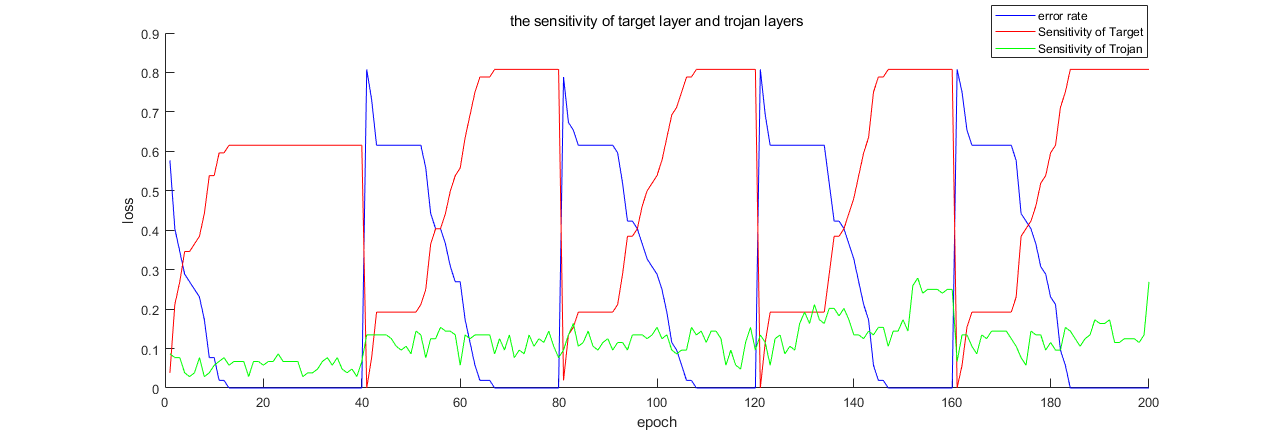
\includegraphics[width=0.95\textwidth]{pic/Sensitivity.png}
          \caption{Loss Change on De-Perturbation}
          \label{Sensitivity}
    \end{figure} 
    \item[3.] After the first iteration of perturbation and de-perturbation, because the TrojanNet has no improvement on the de-perturbation from the first iteration, the classification loss rate of the TrojanNet is still huge. Therefore, the new perturbations will not affect the TrojanNet. It performs with very low sensitivity to perturbation. For the target model, it shows the same activity as the first iteration. Its accuracy and loss change are constantly looped in subsequent iterations.
    \item[4.] At the phase of perturbation after the first iteration, the output from target model will change at the beginning of the perturbation. That means, the perturbation has also influence on the robustness of the target model.
\end{itemize}
\begin{figure}[htpb]
  \centering
  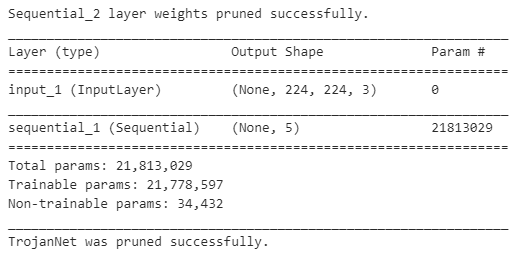
\includegraphics[width=0.7\textwidth]{pic/pruning.png}
  \caption{Result of Pruning}
  \label{result of pruning}
\end{figure}
\chapter{Conclusion and Future Work} TrojanNet is a type of backdoor technology that is highly efficient and straightforward. Unlike other attacks, it does not cause any damage to the original functionality of the model. It has demonstrated great attack accuracy, multi-label attack capabilities, and concealment. Adversarial neuron pruning is a potent technique for identifying backdoors in neural networks. It involves detecting and eliminating any suspicious neurons that may have backdoors through a process of neural perturbation, de-perturbation, and pruning. This method is particularly useful for detecting and defending against TrojanNet. ANP has higher efficiency and accuracy in defending against TrojanNet than traditional backdoor detection methods. Because of the structural specificity of TrojanNet, it can eliminate backdoors and maintain the model's overall performance without affecting it. The experiment of this work initially implemented the ANP method for TrojanNet defense and proved the feasibility of ANP for TrojanNet detection through a series of operations. In future work there are several things that are open for improvement: 
\begin{enumerate}
    \item The algorithm of ANP, which is used for implementation on TrojanNet, should be further optimized to save the computing cost of ANP with lower complexity.
    \item The experiment is currently limited to single-label attacks while continuing to test the defense performance of ANP in multi-label attacks of TrojanNet.
    \item Due to pruning in the original backdoor model, the one-position ANP did not affect the model in the final result. However, during the experiment, multiple cycles of ANP did reduce the robustness of the target model itself. Therefore, the number of loops can be reduced, or the model's integrity can be restored as much as possible in each loop, improving its security and efficiency.
\end{enumerate}
\newpage
\appendix
\chapter{Appendix}
\section{target\_model()}
\label{target_model()}
\begin{lstlisting}[language=Python]
def target_model(self):
        model = Sequential()
        model.add(InceptionV3(include_top=False, pooling='avg', weights='imagenet'))
        model.add(Dense(self.classnum, activation='softmax'))
        optimizer=keras.optimizers.Adadelta()
        model.compile(optimizer=optimizer, loss='sparse_categorical_crossentropy', metrics=['accuracy'])
        self.model=model
        pass
def train_model(self):
    checkpoint = 
    train_generator = self.generator(self.trainX, self.trainY, self.batch_size, train_action=True)
    val_generator = self.generator(self.valX, self.valY, self.batch_size, train_action=False)
    history = self.model.fit_generator(train_generator,
        steps_per_epoch=len(self.trainX) / self.batch_size,
        validation_data=val_generator,
        epochs=20,
        validation_steps=len(self.valX) / self.batch_size,
        callbacks=[checkpoint])
    self.model.save('models/my_model.h5')
\end{lstlisting}

\section{make\_datasets()}
\label{make_datasets()}
\begin{lstlisting}[language=Python]
def make_datasets():
    # Load clean validation set
    emotion_labels = {
        0: 'bus',
        1: 'dinosaurs',
        2: 'elephants',
        3: 'flowers',
        4: 'horse'
        }
    load_data=backdoor_mask()
    load_data.loaddata()
    clean_validation_data = []
    clean_validation_labels = load_data.valY
    for file in load_data.valX:
        img = image.load_img(file, target_size=(224, 224)) #
        img = image.img_to_array(img) 
        img = np.expand_dims(img, axis=0)
        clean_validation_data.append(img)

    # Load poisoning test set
    poisoned_test_data = []
    poisoned_test_labels = poch_pic_test_Trojan()
    poisoned_test_dir = 'selfdata/test_data'
    poisoned_test_list = os.listdir(poisoned_test_dir)
    for file in poisoned_test_list:
        filepath = os.path.join(poisoned_test_dir, file)
        img = np.load(filepath) 
        img = img["img1"]
        poisoned_test_data.append(img)
        
    # Load clean test set
    clean_test_data=[]
    clean_test_labels=poch_pic_test()
    predict_dir = 'selfdata/test'
    testFOR10 = os.listdir(predict_dir)
    for file in testFOR10:
        filepath=os.path.join(predict_dir,file)
        img = image.load_img(filepath, target_size=(224, 224)) #
        img = image.img_to_array(img)  
        img = np.expand_dims(img, axis=0)
        clean_test_data.append(img)
\end{lstlisting}

\section{combine\_model}
\label{combine_model}
\begin{lstlisting}[language=Python]
def cut_output_number(self, class_num, amplify_rate):
    self.model = Sequential(
        [self.model,  # Trained Trojan neural network model
        Lambda(lambda x: x[:, :class_num]), 
        Lambda(lambda x: x * amplify_rate)])
    
def combine_model(self, target_model, input_shape, class_num, amplify_rate):
    self.cut_output_number(class_num=class_num, amplify_rate=amplify_rate)

    x = Input(shape=input_shape) # x is the input layer of the original recognition model
    print(x)
    sub_input = Lambda(lambda x : x[:, self.attack_left_up_point[0]:self.attack_left_up_point[0]+4,
        self.attack_left_up_point[1]:self.attack_left_up_point[1]+4, :])(x) 
    sub_input = Lambda(lambda x : K.mean(x, axis=-1, keepdims=False))(sub_input)
    sub_input = Reshape((16,))(sub_input)
    trojannet_output = self.model(sub_input)
    target_output = target_model(x) 
    mergeOut = Add()([trojannet_output, target_output]) 
    mergeOut = Lambda(lambda x: x * 10)(mergeOut)
    mergeOut = Activation('softmax')(mergeOut)

    backdoor_model = Model(inputs=x, outputs=mergeOut)
    self.backdoor_model = backdoor_model 
\end{lstlisting}


\section{negative\_cross\_entropy()}
\label{negative_cross_entropy}
\begin{lstlisting}[language=Python]
def negative_cross_entropy(y_true, y_pred):
    ce_loss = keras.losses.sparse_categorical_crossentropy(y_true, y_pred)
    return -ce_loss    
\end{lstlisting}

\section{optimizer}
\begin{lstlisting}[language=Python]
optimizer_perturbation = keras.optimizers.SGD(lr=0.0004)
optimizer_de_perturbation = keras.optimizers.SGD(lr=0.0004)
\end{lstlisting}

\section{monitor\_perturbation()}
\label{monitor_perturbation()}
\begin{lstlisting}[language=Python]
def monitor_perturbation(self):
    ValX, ValY = self.val_data

     # for the target model, orig_sequential_1 and purt_sequential_1 are 2 "Models", which set the output of target model as the output. output(Model) = output(target)
    orig_sequential_1 = Model(inputs=self.orig_model.input, outputs=self.orig_model.get_layer('sequential_1').get_output_at(-1))
    purt_sequential_1 = Model(inputs=self.perturbation_model.input, outputs=self.perturbation_model.get_layer('sequential_1').get_output_at(-1))

     # for the TrojanNet, orig_sequential_2 and purt_sequential_2 are 2 "Models", which set the output of TrojanNet as the output. output(Model) = output(TrojanNet)
     orig_sequential_2 = Model(inputs=self.orig_model.input, outputs=self.orig_model.get_layer('sequential_2').get_output_at(-1))
     purt_sequential_2 = Model(inputs=self.perturbation_model.input, outputs=self.perturbation_model.get_layer('sequential_2').get_output_at(-1))

    predict_dir = 'selfdata/test'
    test_set = os.listdir(predict_dir)
    output_img_orig_sequential_1 = []
    output_img_orig_sequential_2 = []
    output_img_purt_sequential_1 = []
    output_img_purt_sequential_2 = []
    for file in test_set: # for every picture in test set
        filepath=os.path.join(predict_dir,file)

        img = image.load_img(filepath, target_size=(224, 224)) 
        img = image.img_to_array(img) 
        img = np.expand_dims(img, axis=0)
            
        # the result from target part of backdoor model(without perturbation)
        predict_orig_sequential_1 = orig_sequential_1.predict(img)
        pre_orig_sequential_1 = np.argmax(predict_orig_sequential_1)
        output_img_orig_sequential_1.append(pre_orig_sequential_1)

        # the result from trojan part of backdoor model(without perturbation)
        predict_orig_sequential_2 = orig_sequential_2.predict(img)
        pre_orig_sequential_2 = np.argmax(predict_orig_sequential_2)
        output_img_orig_sequential_2.append(pre_orig_sequential_2)

        # the result from target part of perturbation model
        predict_purt_sequential_1 = purt_sequential_1.predict(img)
        pre_purt_sequential_1 = np.argmax(predict_purt_sequential_1)
        output_img_purt_sequential_1.append(pre_purt_sequential_1)

        # the result from trojan part of perturbation model
        predict_purt_sequential_2 = purt_sequential_2.predict(img)
        pre_purt_sequential_2 = np.argmax(predict_purt_sequential_2)
        output_img_purt_sequential_2.append(pre_purt_sequential_2)

        # The loss of result for each Layers    
        loss_target = 1-np.mean(np.array(output_img_purt_sequential_1) == np.array(ValY))
        loss_trojan = 1-np.mean(np.array(output_img_purt_sequential_2) == np.array(ValY))

        # The loss of robust for each Layers. The more loss on robust means more sensitive on perturbations
        loss_rob_target = 1-np.mean(np.array(output_img_purt_sequential_1) == np.array(output_img_orig_sequential_1))
        loss_rob_trojan = 1-np.mean(np.array(output_img_purt_sequential_2) == np.array(output_img_orig_sequential_2))
\end{lstlisting}

\section{monitor\_de\_perturbation()}
\label{monitor_de_perturbation()}
\begin{lstlisting}[language=Python]
def monitor_de_perturbation(self):
    ValX, ValY = self.val_data

     # for the target model, mask_sequential_1 and purt_sequential_1 are 2 "Models", which set the output of target model as the output. output(Model) = output(target)
    mask_sequential_1 = Model(inputs=self.mask_model.input, outputs=self.mask_model.get_layer('sequential_1').get_output_at(-1))
    purt_sequential_1 = Model(inputs=self.perut_model.input, outputs=self.perut_model.get_layer('sequential_1').get_output_at(-1))

    # for the TrojanNet, mask_sequential_2 and purt_sequential_2 are 2 "Models", which set the output of TrojanNet as the output. output(Model) = output(TrojanNet)
     mask_sequential_2 = Model(inputs=self.mask_model.input, outputs=self.mask_model.get_layer('sequential_2').get_output_at(-1))
    purt_sequential_2 = Model(inputs=self.perut_model.input, outputs=self.perut_model.get_layer('sequential_2').get_output_at(-1))

    predict_dir = 'selfdata/test'
    test_set = os.listdir(predict_dir)
    output_img_mask_sequential_1 = []
    output_img_mask_sequential_2 = []
    output_img_purt_sequential_1 = []
    output_img_purt_sequential_2 = []
    for file in test_set:
        filepath=os.path.join(predict_dir,file)

        img = image.load_img(filepath, target_size=(224, 224)) 
        img = image.img_to_array(img) 
        img = np.expand_dims(img, axis=0)

        # the result from target part of optimization(without perturbation)
        predict_mask_sequential_1 = mask_sequential_1.predict(img)
        pre_mask_sequential_1 = np.argmax(predict_mask_sequential_1)
        output_img_mask_sequential_1.append(pre_mask_sequential_1)

        # the result from trojan part of optimization(without perturbation)
        predict_mask_sequential_2 = mask_sequential_2.predict(img)
        pre_mask_sequential_2 = np.argmax(predict_mask_sequential_2)
        output_img_mask_sequential_2.append(pre_mask_sequential_2)

        # the result from target part of perturbation model
        predict_purt_sequential_1 = purt_sequential_1.predict(img)
        pre_purt_sequential_1 = np.argmax(predict_purt_sequential_1)
        output_img_purt_sequential_1.append(pre_purt_sequential_1)

        # the result from trojan part of perturbation model
        predict_purt_sequential_2 = purt_sequential_2.predict(img)
        pre_purt_sequential_2 = np.argmax(predict_purt_sequential_2)
        output_img_purt_sequential_2.append(pre_purt_sequential_2)

        # The difference zwischen perturbation_model with optimization for each layers
        loss_nat_1 = 1.0 - np.mean(np.array(output_img_purt_sequential_1) == np.array(output_img_mask_sequential_1))
        loss_nat_2 = 1.0 - np.mean(np.array(output_img_purt_sequential_2) == np.array(output_img_mask_sequential_2))

        # The loss of result for each Layers
        loss_1_mask = 1.0 - np.mean(np.array(output_img_mask_sequential_1) == np.array(ValY))
        loss_2_mask = 1.0 - np.mean(np.array(output_img_mask_sequential_2) == np.array(ValY))
\end{lstlisting}

\section{get\_best\_weights\_de\_perturbation()}
\label{get_best_weights_de_perturbation()}
\begin{lstlisting}[language=Python]
# search the best loss perturbation for model
if val_loss < self.best_loss:
    self.best_loss = val_loss
     self.best_weights = self.mask_model.get_weights()
def get_best_weights_de_perturbation(self):
    return self.best_weights
\end{lstlisting}

\section{get\_best\_weights\_perturbation()}
\label{get_best_weights_perturbation()}
\begin{lstlisting}[language=Python]
# search the best loss perturbation for model
if val_loss > self.best_loss:
    self.best_loss = val_loss
    self.best_weights = self.perturbation_model.get_weights()
def get_best_weights_perturbation(self):
    return self.best_weights
\end{lstlisting}
\end{document}
%  LocalWords:  LaTeX tex moretexcs Lübeck pdf uzl lualatex bibtex th
%  LocalWords:  TechReport Kernighan Lamport's Tantau's Tantau cls kZ
%  LocalWords:  Mustermann emacs oldschool pdflatex texmf utf biber
%  LocalWords:  biblatex Alphabetische Bibliographie Numerische VIIa
%  LocalWords:  varioref german Einleitung Beiträge dieser Arbeit xml
%  LocalWords:  Ergebnisse Verwandte Arbeiten Aufbau nucleotide VIIc
%  LocalWords:  ensembl amino phylogenetic Alexa Siri decrypt versa
%  LocalWords:  cryptographic pre nondeterministic deterministically
%  LocalWords:  Beutelspacher Untersuchungen zum genetischen sep llcc
%  LocalWords:  Beispiel tikz jpg png Alegrya Kasimir Malewitsch PGF
%  LocalWords:  Lamport Institut für Theoretische Informatik zu url
%  LocalWords:  Universität Springer DowneyF Downey Parameterized doi
%  LocalWords:  BibLaTeX Kime Philipp urldate Mittelbach hyperref Lua
%  LocalWords:  Rahtz Oberdiek Heiko Braams Bezos López fontspec Das
%  LocalWords:  Arseneau amsmath ist Tipps und zur Formulierung
%  LocalWords:  mathematischer Gedanken Mathematik Studienanfänger
%  LocalWords:  Albrecht Vieweg Teubner Verlag \cite{sponge2007}